\chapter{Design}\label{ch:Design} %software architecture0,
The design of a robotic prosthesis system for a user having a shoulder disarticulation can be quite comprehensive. This report will strive to create a proof of concept fulfilling the requirements, showing that the use of a robotic limb has the potential to assist a user in a daily task.

\section{General design solution}
The solution to the problems presented in Chapter \ref{ch:FinalProb} is presented in the following section. In order to comply with the technical requirements a solution must have certain components.

\subsection*{Robot manipulator}
An electrical prosthesis is based around a robotic manipulator. The robotic manipulators have several variables needed to be considered when choosing witch one to base the prosthesis design on. To satisfy requirement \ref{req:extension}, the manipulator needs to be able to carry $0.5 kg$. When fully extended and have an end-effector while being small enough to be plausibly attachable to a user.

\subsection*{EMG detection unit}
To control the manipulator, the user would need a control method, as mentioned in chapter \ref{Control} the use of EMG sensors would be ideal for the user. The EMG sensors use the muscle contractions as a signal, that changes depending on the contraction intensity. As the signal intensity changes depending on the contraction, certain thresholds needs to be created in order to satisfy Requirement \ref{req:EMGfatigue} while eliminating the risk of  muscles at rest activating the manipulator. 
\\

A short introduction to sEMG was given in the control systems section \ref{sEMG}. A more detailed description on how to make input control system from the sEMG can be found later in the report.

\paragraph{Electromyography} or EMG. as it has been called throughout this project, is a visualisation of the sum of difference in the potential measured fibres within one muscle. A skeletal muscle is made up of many small fibres called myofibril that each produces a difference in the potential. This signal needs amplification furthermore the signal has to be processed with the help of the analogue process, as described later in the section, in order to create a reliable source of control. The use of EMG is well documented in different articles in the use of a prosthetic arm  \cite{Castellini2009}. The EMG signal in this report is used to describe the signal that is being interpret.

\subsection*{Signal processing}
When the control unit receives the sEMG data, either through a micro-controller or a computer that processes the data, the data is the raw input data from the sEMG and cannot be used as an input for a control system. It is therefore clear that there is a need for processing the received data. In this project the signal is analysed through method of root mean square(RMS) which is an implemented part of the hardware, this is described later in this section.
\\ 

\subsubsection{Filters}
Digital filters is an important part of signal processing. 
These filters removes the noise in the signal depending on what frequencies of the signal that is useful for a robot or radio. A robot needs low frequencies due to it being a mechanical system.\\
Filters are classified as the frequency types it will filter on the signal. Two of the filters, the \textbf{low-pass} and the \textbf{high-pass} describes the filters that let the signal pass above or below a certain cutoff frequency. There is also the band-pass, and the band-stop filter which let the frequency's in a defined bandwidth pass through or block them respectively.
The most suited filter should be chosen based on analysis of the signal.

\paragraph{Sampling}
Certain precautions needs to be taken when sampling the sEMG signal. according to the \textit{Nyquist theorem} the sampling rate should be at least twice that of the signal frequency in order to insure the sinusoid of the EMG signal can be recreated. If this is not done then the data could be corrupted by the aliasing phenomenon. \cite{Nyquist}

%there are in general two use categorys, \textit{signal separation} and \textit{signal restoration}. \cite{FilterBa67:online}


%\paragraph{Signal separation} as the name implies this category seperates the signal passed through. this is normally used when the signal is contaminated with signal noise or other interference. in praxis an example could be a muscle sensor on the pectoralis major. here the signal might be contaminated with noise from the heart or other muscles. 
%therefore there would be a need to seperate the signals and isolate the wanted muscle signal.\cite{FilterBa67:online}
%\paragraph{signal restoration} this refers to when a signal has been distorted. an example could be an audio recording. after filtering it, the sound quality might improve beyond the original. \cite{FilterBa67:online}

\subsection*{Electronic hardware} \label{sec:elHW}
For a signal to be used in a software application there is a need for a way to interpret the signal. In this project the use of an EMG signal requires a hardware part, in this case, it is the muscle sensor v 3.0 from Advancer technology. The muscle sensor measures the signal through the electrodes placed on the user, furthermore, the device amplifies the signal by a gain of 100, it also rectifies the wave signal, which will be described later. The EMG sensor smooths the signal and convert it from an analogue signal to a digital signal that can be processed\cite{EMGHARD}.\\
As seen in figure: \ref{fig:GainsEMG}, the gain is decided through resistor R1, the voltage goes through MID and END, which are EMG inputs. The EMG signals then get amplified across the operational amplifier(OP AMP).\\

\begin{multicols}{2}  
\begin{figure}[H]
    \centering
    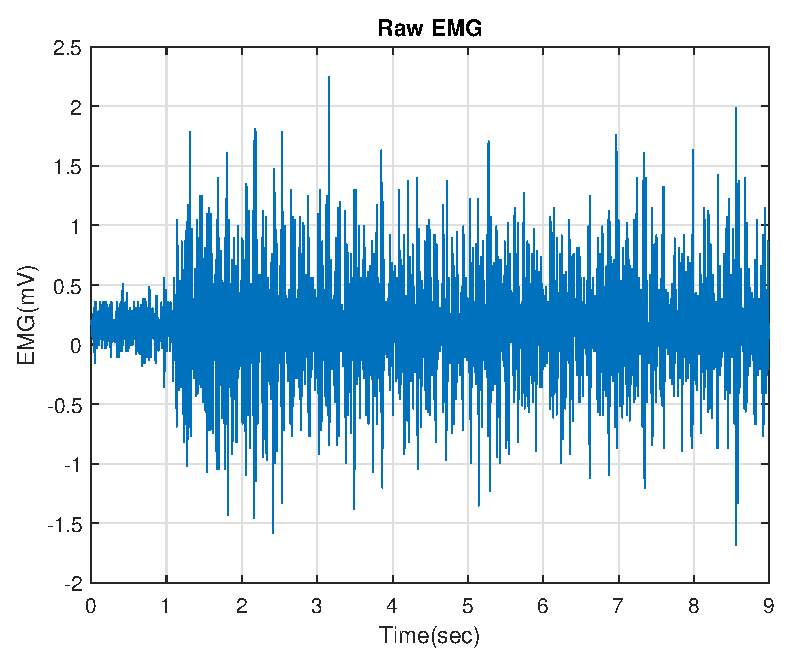
\includegraphics[width=0.4\textwidth]{Figures/EMG/epsFigRAW}
    \caption{\centering{EMG in a raw form analysed \\through matlab, data was borrow from\cite{EMGDATA}}}
\end{figure} 
\columnbreak
\begin{figure}[H]
    \centering
    \includegraphics[width=0.4\textwidth]{Figures/EMG/AmpGB.PNG}
    \caption{\centering{The schematics of the gain of the sEMG signal}\cite{SparkfunScematicEMG}}
    \label{fig:GainsEMG}
\end{figure} 
\end{multicols}

\paragraph{Full wave}
rectifying can be done by hardware or software. The software approach can be done simply by taking the absolute value  of the input data, in this case the hardware rectify the wave\cite{RMS}. Since the signal is an alternating waveform the signal is now only represented as positive numbers. Furthermore, the negative part of the data-set is conserved by squaring the value. This is important for the next step in analysing the data signal, and the root mean square process.\\
The schematics of rectifying the signal can be seen in \ref{fig:rect}, has a input from the latest schematic "Measure", where it polarises the input through a capacitor, and send the polarised signal through a 150k resistor. The signal is then sent through a serial connection, connected with junctions which includes known OP AMP's and ground inputs. The signal is now rectified.\\

\begin{multicols}{2}
\begin{figure}[H]
    \centering
   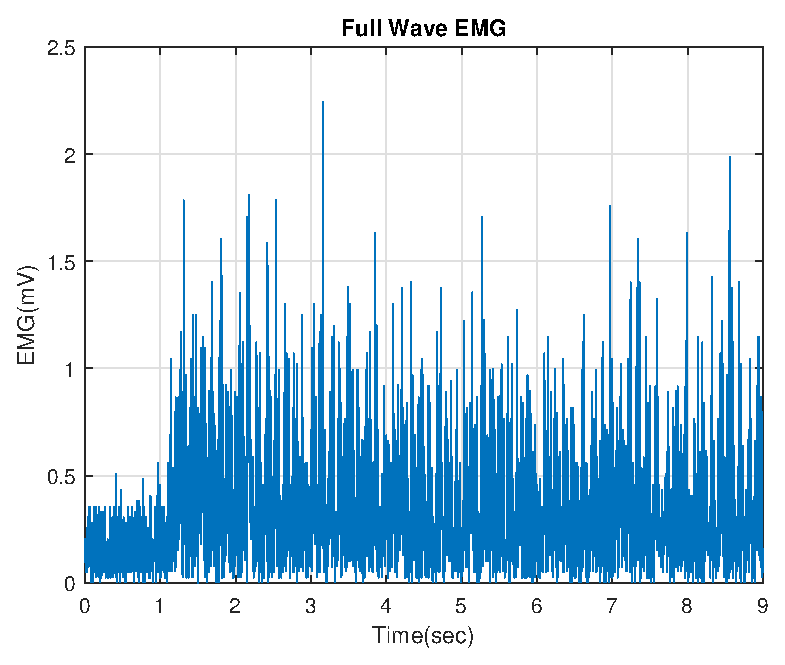
\includegraphics[width=0.3\textwidth]{Figures/EMG/epsFig}
    \caption{\centering{ EMG in Full wave form analysed \\through Matlab, data was borrow from \cite{EMGDATA}}}
\end{figure} 
\columnbreak
\begin{figure}[H]
    \centering
    \includegraphics[width=0.7\textwidth]{Figures/EMG/Rect.PNG}
    \caption{\centering{The schematics of the rectifying on the EMG sensors}\cite{SparkfunScematicEMG}}
    \label{fig:rect}
\end{figure} 
\end{multicols} 
\paragraph{Root mean square} or RMS is a solution made in order to get an average over time from any signal. It needs the wave form described in the full wave, this is referring to the squared part of RMS, so the means of the EMG signal can be evaluated, refraining from the rectifying of the squared part gets the mean of zero\cite{RMS}. After processing the signal it
is used as an implementation for a control signal.\\
The next step of schematics is as seen in \ref{fig:smooth}, is smoothing out the signal as described above. The rectified signal gets processed in a serial connection with known OP AMP's, resistors and capacitors. When the EMG signal is sent through this part of EMG sensor, the signal is smoothed.\\
The last schematics \ref{fig:finalGain}, with smooth signal as input, it is again put through a OP AMP to get the last gain before the signal is converted into a digital representation of the signal. The gain in this OP AMP is decided through the potentiometer.\\


\begin{multicols}{2}
\begin{figure}[H]
    \centering
    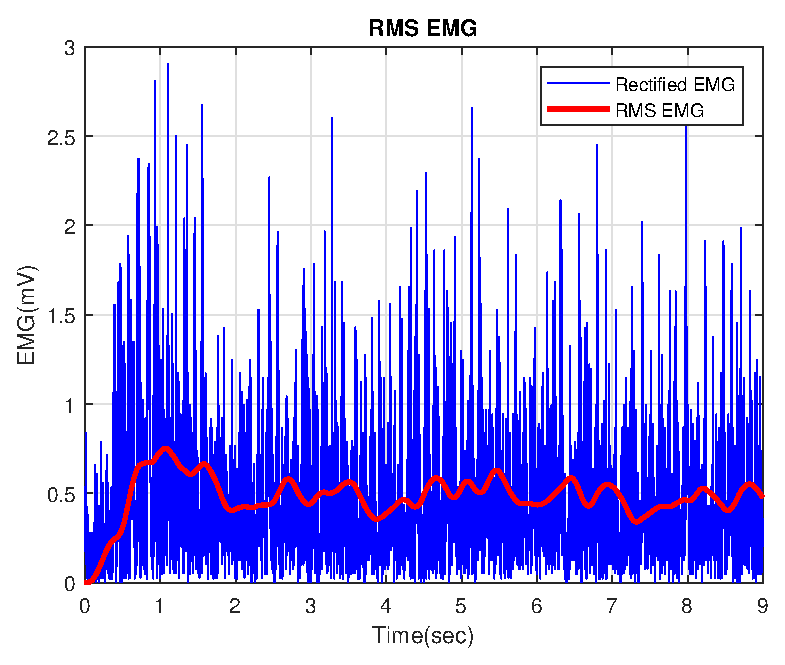
\includegraphics[width=0.4\textwidth]{Figures/EMG/epsFigRMS}
    \caption{EMG in Full wave with RMS analyses\\ preformed in matlab, data was borrow from\cite{EMGDATA}}
    \label{ref:Wasmooth}
\end{figure}
\columnbreak
\begin{figure}[H]
    \centering
    \includegraphics[width=0.4\textwidth]{Figures/EMG/Smooth.PNG}
    \caption{The schematics of the smoothing on the EMG sensors\cite{SparkfunScematicEMG}}
    \label{fig:smooth}
\end{figure} 
\end{multicols}




\begin{figure}[H]
    \centering
    \includegraphics[width=0.5\textwidth]{Figures/EMG/FinalGain.PNG}
    \caption{\centering{The schematics of the last gain on the EMG sensors before data is transmitted\cite{SparkfunScematicEMG}}}
    \label{fig:finalGain}
\end{figure} 


\subsection*{Muscle choice}
 Any distinct muscles which can voluntarily be controlled by the user could, in theory, be used as the input to the control system. Examples of possible choices could be the use of facial muscles, or the use of the muscles from the remaining arm. Surgically attaching the muscles closer to the skin to get a better signal is also an option \cite{SimonsSu49:online}.\\
 Difficulties in receiving a stable signal will change depending on the electrodes location on the body, e.g the breast muscles on the upper torso. The torso-muscles could be an ideal choice for some users, but if the electrodes were to be placed close to the heart, the heart-rhythm could interfere with the signal, while heightening the difficulties in receiving a stable control signal, due to the added noise from the heart, and would need to be filtered out. \\
 As a proof of concept the muscles in the lower arm as seen in figures \ref{ref:UpperArm} and \ref{fig:UnderArm} is used due to their accessible location when placing the electrodes while testing.
\begin{multicols}{2}
\begin{figure}[H]
    \centering
    \includegraphics[width=0.4\textwidth]{Figures/Technical_figures/OverArm.jpg}
    \caption{Picture showing the placement of electrodes on top of the forearm, where the green electrode is the neutral point, and both the black and red electrodes are placed on the same muscle}
    \label{ref:UpperArm}
\end{figure}
\columnbreak
\begin{figure}[H]
    \centering
    \includegraphics[width=0.4\textwidth]{Figures/Technical_figures/UnderArm.jpg}
    \caption{Figure showing the placement of electrodes under the forearm, where green is the neutral point, and both black and red is on the same muscle}
    \label{fig:UnderArm}
\end{figure} 
\end{multicols}

\subsection*{Inertial measuring unit}% kort generelt omkring IMu og gyro og hvordan det kan bruges
 In order supplement the EMG detection unit, an IMU with an accelerometer and/or a gyroscope can be used to control a manipulator by utilising a change in either orientation or acceleration. This can be done by attaching the IMU to a body-part on the user and having them move said body-part in a predetermined x, y or z-direction. An example could be placing the module on the users head or shoulder and having them accelerating it in a direction specified. This change in acceleration could then be used to change the motor chosen, or the motors angle depending on the degree of unit tilt or if the acceleration measured exceeded a preset threshold.

\subsection*{Radio module}
Requirement \ref{req:electrocution} specifies the user not being attached to the manipulator in order to remove the risk of the user being electrocuted. By definition there is a need to transmit between the user and the manipulator wireless, therefore a radio module would be needed. However according to requirement \ref{test:Latency} the latency experienced by the user when operating the manipulator cannot exceed one second. The requirements of the radio modules would therefore need a fast rate of data transmission between the modules for the user not to experience a lag in control of the manipulator.

\subsection*{PC/Micro-controller}
To control the data transmitted it has to be interpreted and converted into a manipulator movement by a computer. The computer would work as the systems "brain" and could operate in several ways. One option could be to use a laptop to receive data from the sensors while computing and transmitting the data to a micro-controller attached to the manipulator. Another option could be for the micro-controller itself to receive the data from the sensors and directly move the manipulator without the need of an attached laptop. 
\subsubsection*{Control Systems}
%Intro:
The control system takes the input signal and use it to gain the desired output. By this definition the system could  e.g, take the signal of a muscle contraction and translate it into a motor angle change change.
\begin{figure}[H]
    \centering
    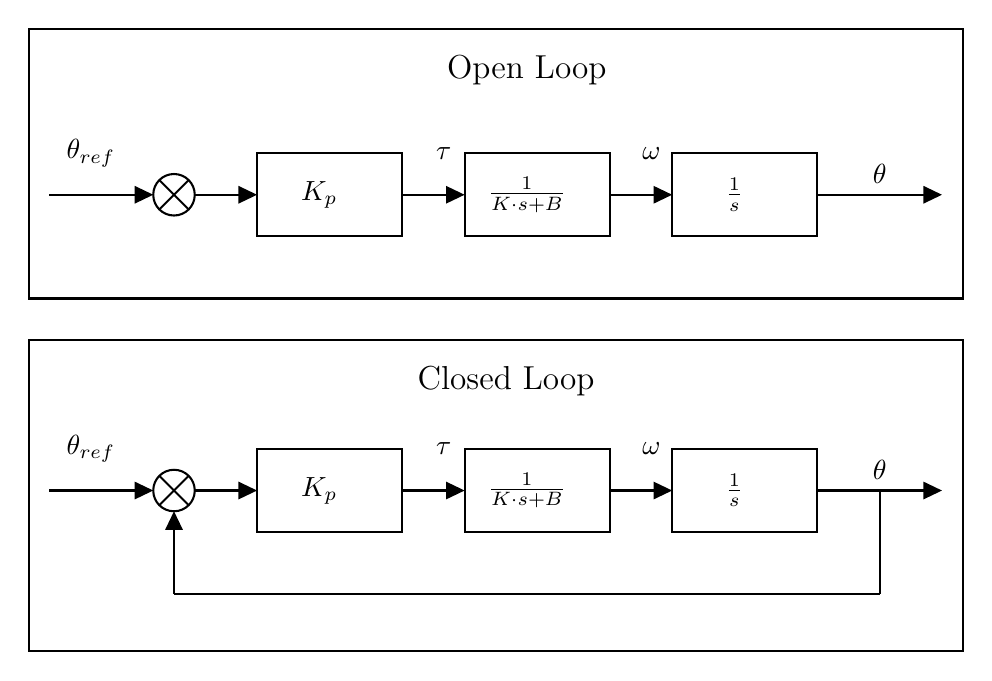
\begin{tikzpicture}[x=0.75pt,y=0.75pt,yscale=-1,xscale=1]
%uncomment if require: \path (0,328.50892877578735); %set diagram left start at 0, and has height of 328.50892877578735

%Shape: Rectangle [id:dp12482796861282974] 
\draw   (140,80) -- (210,80) -- (210,120) -- (140,120) -- cycle ;
%Straight Lines [id:da5706724332227189] 
\draw    (40,100) -- (88,100) ;
\draw [shift={(90,100)}, rotate = 180] [fill={rgb, 255:red, 0; green, 0; blue, 0 }  ][line width=0.75]  [draw opacity=0] (8.93,-4.29) -- (0,0) -- (8.93,4.29) -- cycle    ;

%Flowchart: Summing Junction [id:dp53704430353601] 
\draw   (90,100) .. controls (90,94.48) and (94.48,90) .. (100,90) .. controls (105.52,90) and (110,94.48) .. (110,100) .. controls (110,105.52) and (105.52,110) .. (100,110) .. controls (94.48,110) and (90,105.52) .. (90,100) -- cycle ; \draw   (92.93,92.93) -- (107.07,107.07) ; \draw   (107.07,92.93) -- (92.93,107.07) ;
%Straight Lines [id:da3178828171562029] 
\draw    (110,100) -- (138,100) ;
\draw [shift={(140,100)}, rotate = 180] [fill={rgb, 255:red, 0; green, 0; blue, 0 }  ][line width=0.75]  [draw opacity=0] (8.93,-4.29) -- (0,0) -- (8.93,4.29) -- cycle    ;

%Shape: Rectangle [id:dp28027349651381117] 
\draw   (240,80) -- (310,80) -- (310,120) -- (240,120) -- cycle ;
%Straight Lines [id:da11899224305491352] 
\draw    (210,100) -- (238,100) ;
\draw [shift={(240,100)}, rotate = 180] [fill={rgb, 255:red, 0; green, 0; blue, 0 }  ][line width=0.75]  [draw opacity=0] (8.93,-4.29) -- (0,0) -- (8.93,4.29) -- cycle    ;

%Shape: Rectangle [id:dp31656367205122615] 
\draw   (340,80) -- (410,80) -- (410,120) -- (340,120) -- cycle ;
%Straight Lines [id:da5367106543687827] 
\draw    (310,100) -- (338,100) ;
\draw [shift={(340,100)}, rotate = 180] [fill={rgb, 255:red, 0; green, 0; blue, 0 }  ][line width=0.75]  [draw opacity=0] (8.93,-4.29) -- (0,0) -- (8.93,4.29) -- cycle    ;

%Straight Lines [id:da7913281226659683] 
\draw    (410,100) -- (468,100) ;
\draw [shift={(470,100)}, rotate = 180] [fill={rgb, 255:red, 0; green, 0; blue, 0 }  ][line width=0.75]  [draw opacity=0] (8.93,-4.29) -- (0,0) -- (8.93,4.29) -- cycle    ;

%Shape: Rectangle [id:dp11142722632197088] 
\draw   (30,20) -- (480,20) -- (480,150) -- (30,150) -- cycle ;
%Shape: Rectangle [id:dp14600397799019293] 
\draw   (140,222.5) -- (210,222.5) -- (210,262.5) -- (140,262.5) -- cycle ;
%Straight Lines [id:da4243355948071521] 
\draw    (40,242.5) -- (88,242.5) ;
\draw [shift={(90,242.5)}, rotate = 180] [fill={rgb, 255:red, 0; green, 0; blue, 0 }  ][line width=0.75]  [draw opacity=0] (8.93,-4.29) -- (0,0) -- (8.93,4.29) -- cycle    ;

%Flowchart: Summing Junction [id:dp6729381602093008] 
\draw   (90,242.5) .. controls (90,236.98) and (94.48,232.5) .. (100,232.5) .. controls (105.52,232.5) and (110,236.98) .. (110,242.5) .. controls (110,248.02) and (105.52,252.5) .. (100,252.5) .. controls (94.48,252.5) and (90,248.02) .. (90,242.5) -- cycle ; \draw   (92.93,235.43) -- (107.07,249.57) ; \draw   (107.07,235.43) -- (92.93,249.57) ;
%Straight Lines [id:da14869215035902505] 
\draw    (110,242.5) -- (138,242.5) ;
\draw [shift={(140,242.5)}, rotate = 180] [fill={rgb, 255:red, 0; green, 0; blue, 0 }  ][line width=0.75]  [draw opacity=0] (8.93,-4.29) -- (0,0) -- (8.93,4.29) -- cycle    ;

%Shape: Rectangle [id:dp9900763090446374] 
\draw   (240,222.5) -- (310,222.5) -- (310,262.5) -- (240,262.5) -- cycle ;
%Straight Lines [id:da7760938350165698] 
\draw    (210,242.5) -- (238,242.5) ;
\draw [shift={(240,242.5)}, rotate = 180] [fill={rgb, 255:red, 0; green, 0; blue, 0 }  ][line width=0.75]  [draw opacity=0] (8.93,-4.29) -- (0,0) -- (8.93,4.29) -- cycle    ;

%Shape: Rectangle [id:dp19026495853512104] 
\draw   (340,222.5) -- (410,222.5) -- (410,262.5) -- (340,262.5) -- cycle ;
%Straight Lines [id:da42905616589605233] 
\draw    (310,242.5) -- (338,242.5) ;
\draw [shift={(340,242.5)}, rotate = 180] [fill={rgb, 255:red, 0; green, 0; blue, 0 }  ][line width=0.75]  [draw opacity=0] (8.93,-4.29) -- (0,0) -- (8.93,4.29) -- cycle    ;

%Straight Lines [id:da668486289799261] 
\draw    (410,242.5) -- (468,242.5) ;
\draw [shift={(470,242.5)}, rotate = 180] [fill={rgb, 255:red, 0; green, 0; blue, 0 }  ][line width=0.75]  [draw opacity=0] (8.93,-4.29) -- (0,0) -- (8.93,4.29) -- cycle    ;

%Straight Lines [id:da5740200387655516] 
\draw    (100,254.5) -- (100,292.5) ;

\draw [shift={(100,252.5)}, rotate = 90] [fill={rgb, 255:red, 0; green, 0; blue, 0 }  ][line width=0.75]  [draw opacity=0] (8.93,-4.29) -- (0,0) -- (8.93,4.29) -- cycle    ;
%Straight Lines [id:da1492709801617349] 
\draw    (100,292.5) -- (440,292.5) ;


%Straight Lines [id:da5671703763154259] 
\draw    (440,242.5) -- (440,292.5) ;


%Shape: Rectangle [id:dp043811444149466805] 
\draw   (30,170) -- (480,170) -- (480,320) -- (30,320) -- cycle ;

% Text Node
\draw (60,80) node   {$\theta _{ref}$};
% Text Node
\draw (170,100) node   {$K_{p}$};
% Text Node
\draw (230,80) node   {$\tau $};
% Text Node
\draw (270,100) node   {$\frac{1}{K\cdot s+B}$};
% Text Node
\draw (370,100) node   {$\frac{1}{s}$};
% Text Node
\draw (330,80) node   {$\omega $};
% Text Node
\draw (440,90) node   {$\theta $};
% Text Node
\draw (270,40) node  [align=left] {{\large Open Loop}};
% Text Node
\draw (60,222.5) node   {$\theta _{ref}$};
% Text Node
\draw (170,242.5) node   {$K_{p}$};
% Text Node
\draw (230,222.5) node   {$\tau $};
% Text Node
\draw (270,242.5) node   {$\frac{1}{K\cdot s+B}$};
% Text Node
\draw (370,242.5) node   {$\frac{1}{s}$};
% Text Node
\draw (330,222.5) node   {$\omega $};
% Text Node
\draw (440,232.5) node   {$\theta $};
% Text Node
\draw (260,190) node  [align=left] {{\large Closed Loop}};


\end{tikzpicture}

    \caption{Open- and closed loop are control schemes and that show how the signal runs through a controller}
    \label{fig:openclose}
\end{figure}
As seen on the figure \ref{fig:openclose} the open loop manages to compute the reference signal so that it is to be equal to the desired output, assuming that the model of the system is perfect. In the case where a disturbance is introduced to the open loop system, the system can not adjust for the disturbance and would produce an unrecognisable error.\\
The closed-loop system/feedback loop can measure the output error and equals it towards the input while gradually minimising the disturbance making the system linear. The error deletion will make the system easier to work with, but this is another section that will be covered in \ref{PID}.\\ 
Utilising these control systems can be done by transfer functions. Transfer functions is the Laplace formulae of the control system design.\\

\paragraph{The Golden Formula}\\
\begin{figure}[H]
    \centering
    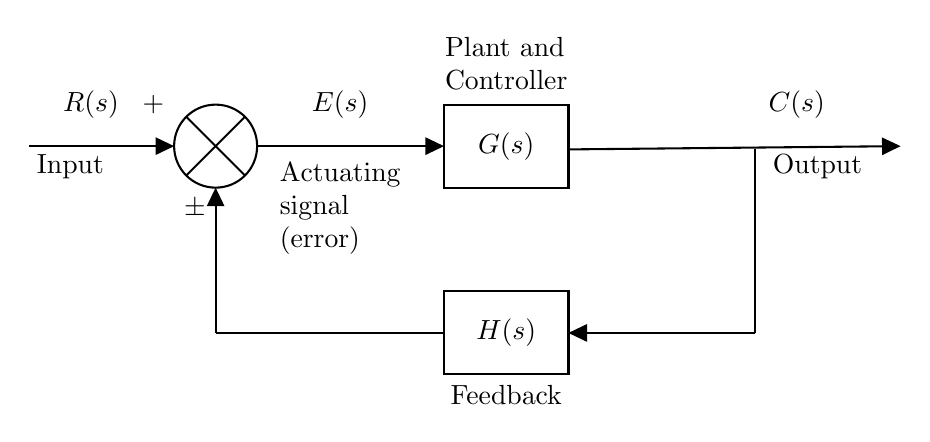
\begin{tikzpicture}[x=0.75pt,y=0.75pt,yscale=-1,xscale=1]
%uncomment if require: \path (0,300); %set diagram left start at 0, and has height of 300

%Straight Lines
\draw    (10,68.71) -- (78,68.71) ;
\draw [shift={(80,68.71)}, rotate = 180] [fill={rgb, 255:red, 0; green, 0; blue, 0 }  ][line width=0.75]  [draw opacity=0] (8.93,-4.29) -- (0,0) -- (8.93,4.29) -- cycle    ;

%Flowchart: Summing Junction
\draw   (80,68.71) .. controls (80,57.67) and (88.95,48.71) .. (100,48.71) .. controls (111.05,48.71) and (120,57.67) .. (120,68.71) .. controls (120,79.76) and (111.05,88.71) .. (100,88.71) .. controls (88.95,88.71) and (80,79.76) .. (80,68.71) -- cycle ; \draw   (85.86,54.57) -- (114.14,82.86) ; \draw   (114.14,54.57) -- (85.86,82.86) ;
%Straight Lines
\draw    (120,68.71) -- (208,68.71) ;
\draw [shift={(210,68.71)}, rotate = 180] [fill={rgb, 255:red, 0; green, 0; blue, 0 }  ][line width=0.75]  [draw opacity=0] (8.93,-4.29) -- (0,0) -- (8.93,4.29) -- cycle    ;

%Shape: Rectangle
\draw   (210,48.71) -- (270,48.71) -- (270,88.71) -- (210,88.71) -- cycle ;
%Straight Lines
\draw    (270,70.29) -- (428,68.73) ;
\draw [shift={(430,68.71)}, rotate = 539.44] [fill={rgb, 255:red, 0; green, 0; blue, 0 }  ][line width=0.75]  [draw opacity=0] (8.93,-4.29) -- (0,0) -- (8.93,4.29) -- cycle    ;

%Straight Lines
\draw    (360,70.29) -- (360,158.71) ;


%Straight Lines
\draw    (360,158.71) -- (272,158.71) ;
\draw [shift={(270,158.71)}, rotate = 360] [fill={rgb, 255:red, 0; green, 0; blue, 0 }  ][line width=0.75]  [draw opacity=0] (8.93,-4.29) -- (0,0) -- (8.93,4.29) -- cycle    ;

%Shape: Rectangle
\draw   (210,138.71) -- (270,138.71) -- (270,178.71) -- (210,178.71) -- cycle ;
%Straight Lines
\draw    (210,158.71) -- (100,158.71) ;


%Straight Lines
\draw    (100,158.71) -- (100,90.71) ;
\draw [shift={(100,88.71)}, rotate = 450] [fill={rgb, 255:red, 0; green, 0; blue, 0 }  ][line width=0.75]  [draw opacity=0] (8.93,-4.29) -- (0,0) -- (8.93,4.29) -- cycle    ;


% Text Node
\draw (40,48.71) node   {$R( s)$};
% Text Node
\draw (70,48.71) node   {$+$};
% Text Node
\draw (160,48.71) node   {$E( s)$};
% Text Node
\draw (240,68.71) node   {$G( s)$};
% Text Node
\draw (380,48.71) node   {$C( s)$};
% Text Node
\draw (240,158.71) node   {$H( s)$};
% Text Node
\draw (90,98.71) node   {$\pm $};
% Text Node
\draw (160,98.71) node  [align=left] {Actuating \\signal\\(error)};
% Text Node
\draw (30,78.71) node  [align=left] {Input};
% Text Node
\draw (390,78.71) node  [align=left] {Output};
% Text Node
\draw (240,188.71) node  [align=left] {Feedback};
% Text Node
\draw (240,28.71) node  [align=left] {Plant and \\Controller};


\end{tikzpicture}
    \caption{Standard format feedback loop here Arrows signify signals and boxes mechanisms, this standard form feedback loop are used to illustrate the golden formula}
    \label{fig:FeedbackLoop}
\end{figure}
When working with the standard setup of a feedback loop the use of the Golden Formula can describe the output $C(s)$ depending on the input $R(s)$.
\begin{equation}\label{eq:GoldenFormula}
    C(s)=\frac{G(s)}{1\mp G(s)\cdot H(s)}\cdot R(s)
\end{equation}
The transfer function given by the Golden Formula, this is called the closed-loop transfer function, the product $G(s)\cdot H(s)$ is called the open-loop transfer-function, or loop-gain. $G(s)$ is the transfer function, while $H(s)$ is difference between input and output, which means that it is the feedback-gain.\\
Transfer functions can be used to establish how various steady-state systems, e.g: "Step-response", "Impulses" or "Ramps", react to viable waveforms.
\paragraph*{Controller design} \label{PID}
There are one specific controller that is related to this project, the PID (Proportional, Integral, Derivative) controller. The PID controller is used to counteract the errors inside a loop. Each of these components drives the error towards zero, which can be read about in the sections to come. Every component has its own allocated gain, a gain can be described as the ratio between the output divided by the input. The objective in this system is to move from one angle to another, the error would then be the difference in angles over time. In this section \textbf{\textit{U}} is denoted as being the effort to be put in the system, which is the controllers amount of power needed to preform its task.\\

\paragraph{Discrete time} In the real world we live in a continues time domain, but computers works in discrete time domain. The discrete time is not measured in seconds, but rather in time frames.\\
The PID controller can ,in theory, find the perfect gains with the most suited rise time and settling time, but in practise this can be an expensive task. The expenses of the system can get high due to the need of a motor that is able to spin and stop at a rate that is suited for the PID controller, and sensors for the system needs to sense the changes within the system at the same rate.\\

\begin{figure} [H]
    \centering
    

\tikzset{every picture/.style={line width=0.75pt}} %set default line width to 0.75pt        

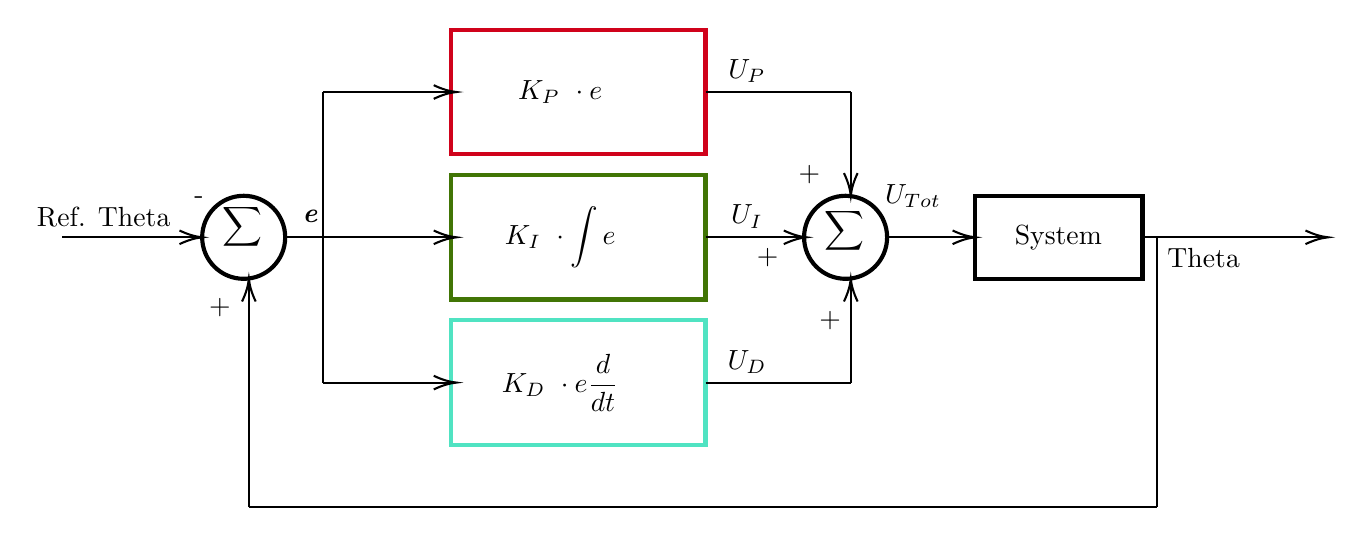
\begin{tikzpicture}[x=0.75pt,y=0.75pt,yscale=-1,xscale=1]
%uncomment if require: \path (0,269); %set diagram left start at 0, and has height of 269

%Shape: Rectangle [id:dp6186698400269734] 
\draw  [color={rgb, 255:red, 208; green, 2; blue, 27 }  ,draw opacity=1 ][line width=1.5]  (217.5,20) -- (340,20) -- (340,80) -- (217.5,80) -- cycle ;
%Shape: Rectangle [id:dp35497397654468] 
\draw  [color={rgb, 255:red, 65; green, 117; blue, 5 }  ,draw opacity=1 ][line width=1.5]  (217.5,90) -- (340,90) -- (340,150) -- (217.5,150) -- cycle ;
%Shape: Rectangle [id:dp0011241398633399236] 
\draw  [color={rgb, 255:red, 80; green, 227; blue, 194 }  ,draw opacity=1 ][line width=1.5]  (217.5,160) -- (340,160) -- (340,220) -- (217.5,220) -- cycle ;
%Shape: Circle [id:dp7081049529214984] 
\draw  [line width=1.5]  (97.5,120) .. controls (97.5,108.95) and (106.45,100) .. (117.5,100) .. controls (128.55,100) and (137.5,108.95) .. (137.5,120) .. controls (137.5,131.05) and (128.55,140) .. (117.5,140) .. controls (106.45,140) and (97.5,131.05) .. (97.5,120) -- cycle ;
%Straight Lines [id:da1012548517194285] 
\draw    (155.61,50) -- (218,50) ;
\draw [shift={(220,50)}, rotate = 180] [color={rgb, 255:red, 0; green, 0; blue, 0 }  ][line width=0.75]    (10.93,-3.29) .. controls (6.95,-1.4) and (3.31,-0.3) .. (0,0) .. controls (3.31,0.3) and (6.95,1.4) .. (10.93,3.29)   ;

%Straight Lines [id:da024552935574742696] 
\draw    (137.5,120) -- (218,120) ;
\draw [shift={(220,120)}, rotate = 180] [color={rgb, 255:red, 0; green, 0; blue, 0 }  ][line width=0.75]    (10.93,-3.29) .. controls (6.95,-1.4) and (3.31,-0.3) .. (0,0) .. controls (3.31,0.3) and (6.95,1.4) .. (10.93,3.29)   ;

%Straight Lines [id:da632489535879416] 
\draw    (155.61,190) -- (218,190) ;
\draw [shift={(220,190)}, rotate = 180] [color={rgb, 255:red, 0; green, 0; blue, 0 }  ][line width=0.75]    (10.93,-3.29) .. controls (6.95,-1.4) and (3.31,-0.3) .. (0,0) .. controls (3.31,0.3) and (6.95,1.4) .. (10.93,3.29)   ;

%Straight Lines [id:da028164362822356237] 
\draw    (155.61,50) -- (155.61,110) ;


%Straight Lines [id:da1783990189247291] 
\draw    (155.61,110) -- (155.61,190) ;


%Shape: Ellipse [id:dp13776991374733094] 
\draw  [line width=1.5]  (387.5,120) .. controls (387.5,108.95) and (396.45,100) .. (407.5,100) .. controls (418.55,100) and (427.5,108.95) .. (427.5,120) .. controls (427.5,131.05) and (418.55,140) .. (407.5,140) .. controls (396.45,140) and (387.5,131.05) .. (387.5,120) -- cycle ;
%Straight Lines [id:da5590648239872058] 
\draw    (340,50) -- (410,50) ;


%Straight Lines [id:da32339100567036794] 
\draw    (340,120) -- (386.65,120) ;
\draw [shift={(388.65,120)}, rotate = 180] [color={rgb, 255:red, 0; green, 0; blue, 0 }  ][line width=0.75]    (10.93,-3.29) .. controls (6.95,-1.4) and (3.31,-0.3) .. (0,0) .. controls (3.31,0.3) and (6.95,1.4) .. (10.93,3.29)   ;

%Straight Lines [id:da37714274354973676] 
\draw    (340,190) -- (410,190) ;


%Straight Lines [id:da12414839144602552] 
\draw    (410,50) -- (410,98) ;
\draw [shift={(410,100)}, rotate = 270] [color={rgb, 255:red, 0; green, 0; blue, 0 }  ][line width=0.75]    (10.93,-3.29) .. controls (6.95,-1.4) and (3.31,-0.3) .. (0,0) .. controls (3.31,0.3) and (6.95,1.4) .. (10.93,3.29)   ;

%Straight Lines [id:da2294854556231043] 
\draw    (410,142) -- (410,190) ;

\draw [shift={(410,140)}, rotate = 90] [color={rgb, 255:red, 0; green, 0; blue, 0 }  ][line width=0.75]    (10.93,-3.29) .. controls (6.95,-1.4) and (3.31,-0.3) .. (0,0) .. controls (3.31,0.3) and (6.95,1.4) .. (10.93,3.29)   ;
%Straight Lines [id:da7636925489142845] 
\draw    (427.5,120) -- (468,120) ;
\draw [shift={(470,120)}, rotate = 180] [color={rgb, 255:red, 0; green, 0; blue, 0 }  ][line width=0.75]    (10.93,-3.29) .. controls (6.95,-1.4) and (3.31,-0.3) .. (0,0) .. controls (3.31,0.3) and (6.95,1.4) .. (10.93,3.29)   ;

%Straight Lines [id:da8120471221631163] 
\draw    (30,120) -- (95.5,120) ;
\draw [shift={(97.5,120)}, rotate = 180] [color={rgb, 255:red, 0; green, 0; blue, 0 }  ][line width=0.75]    (10.93,-3.29) .. controls (6.95,-1.4) and (3.31,-0.3) .. (0,0) .. controls (3.31,0.3) and (6.95,1.4) .. (10.93,3.29)   ;

%Straight Lines [id:da7263862005723072] 
\draw    (120,250) -- (120,142) ;
\draw [shift={(120,140)}, rotate = 450] [color={rgb, 255:red, 0; green, 0; blue, 0 }  ][line width=0.75]    (10.93,-3.29) .. controls (6.95,-1.4) and (3.31,-0.3) .. (0,0) .. controls (3.31,0.3) and (6.95,1.4) .. (10.93,3.29)   ;

%Straight Lines [id:da9777886662003494] 
\draw    (120,250) -- (490,250) ;


%Shape: Rectangle [id:dp7284343716119925] 
\draw  [line width=1.5]  (470,100) -- (550.53,100) -- (550.53,140) -- (470,140) -- cycle ;
%Straight Lines [id:da4771680795774551] 
\draw    (550.53,120) -- (638,120) ;
\draw [shift={(640,120)}, rotate = 180] [color={rgb, 255:red, 0; green, 0; blue, 0 }  ][line width=0.75]    (10.93,-3.29) .. controls (6.95,-1.4) and (3.31,-0.3) .. (0,0) .. controls (3.31,0.3) and (6.95,1.4) .. (10.93,3.29)   ;

%Straight Lines [id:da7739849283065594] 
\draw    (557.37,120) -- (557.37,250) ;


%Straight Lines [id:da5629774692956326] 
\draw    (557.37,250) -- (485.79,250) ;



% Text Node
\draw (50,110) node  [align=left] {Ref. Theta};
% Text Node
\draw (510,120) node  [align=left] {System};
% Text Node
\draw (270,190) node  [align=left] {$\displaystyle K_{D} \ \cdot e  \frac{d}{dt}$};
% Text Node
\draw (270,120) node  [align=left] {$\displaystyle K_{I} \ \cdot \int e$};
% Text Node
\draw (270,50) node  [align=left] {$\displaystyle K_{P} \ \cdot e$};
% Text Node
\draw (390,90) node  [align=left] {+};
% Text Node
\draw (370,130) node  [align=left] {+};
% Text Node
\draw (400,160) node  [align=left] {+};
% Text Node
\draw (106,154) node  [align=left] {+};
% Text Node
\draw (96,101) node  [align=left] {\mbox{-}};
% Text Node
\draw (150,110) node  [align=left] {\textit{\textbf{e}}};
% Text Node
\draw (407,117) node  [align=left] {$\displaystyle \sum $};
% Text Node
\draw (360,110) node  [align=left] {$\displaystyle U_{I}$};
% Text Node
\draw (360,180) node  [align=left] {$\displaystyle U_{D}$};
% Text Node
\draw (360,40) node  [align=left] {$\displaystyle U_{P}$};
% Text Node
\draw (117,115) node  [align=left] {$\displaystyle \sum $};
% Text Node
\draw (440,100) node  [align=left] {$\displaystyle U_{Tot}$};
% Text Node
\draw (580,130) node  [align=left] {Theta};


\end{tikzpicture}

    %\includegraphics{Figures/Technical_figures/1-25.jpg}
    \caption{Layout of a PID controllers response-equations to eliminate the error}
    \label{fig:mPID}
\end{figure}


\begin{equation}\label{PID}
    U=K_P\cdot\textit{e}+K_I\cdot\int\textit{e}+K_D\cdot\textit{e} \frac{d}{dt}
\end{equation}

\paragraph{The Proportional} gain $K_P$ in eq. \ref{PID} is the gain multiplied with the error(e) resulting in the effort.\\
The larger the gain is, results in a faster rise time, the rise time is the time it takes for the response to get from 10\% to 90\% of the final angle. However this controller can only be used alone when the system can tolerate a constant error in steady state, a steady state error is an error over time that does not diminish. The proportional gain also has a tendency to overshoot the desired value if the gain is too high\cite{Control1DK}.\\

\begin{figure}[H]
    \centering
    \includegraphics[width=\textwidth]{Figures/Technical_figures/PGAIN.png} 
    %

\tikzset{every picture/.style={line width=0.75pt}} %set default line width to 0.75pt        

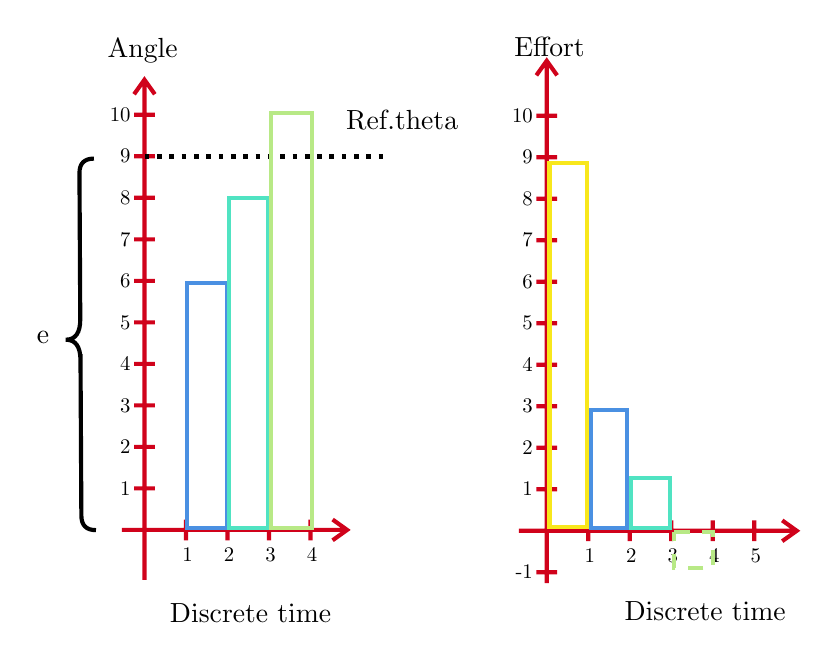
\begin{tikzpicture}[x=0.75pt,y=0.75pt,yscale=-1,xscale=1]
%uncomment if require: \path (0,530); %set diagram left start at 0, and has height of 530

%Shape: Axis 2D [id:dp45682595351826527] 
\draw [color={rgb, 255:red, 208; green, 2; blue, 27 }  ,draw opacity=1 ][line width=1.5]  (90,242.9) -- (198.5,242.9)(100.85,26) -- (100.85,267) (191.5,237.9) -- (198.5,242.9) -- (191.5,247.9) (95.85,33) -- (100.85,26) -- (105.85,33) (120.85,237.9) -- (120.85,247.9)(140.85,237.9) -- (140.85,247.9)(160.85,237.9) -- (160.85,247.9)(180.85,237.9) -- (180.85,247.9)(95.85,222.9) -- (105.85,222.9)(95.85,202.9) -- (105.85,202.9)(95.85,182.9) -- (105.85,182.9)(95.85,162.9) -- (105.85,162.9)(95.85,142.9) -- (105.85,142.9)(95.85,122.9) -- (105.85,122.9)(95.85,102.9) -- (105.85,102.9)(95.85,82.9) -- (105.85,82.9)(95.85,62.9) -- (105.85,62.9)(95.85,42.9) -- (105.85,42.9) ;
\draw   (127.85,254.9) node[anchor=east, scale=0.75]{1} (147.85,254.9) node[anchor=east, scale=0.75]{2} (167.85,254.9) node[anchor=east, scale=0.75]{3} (187.85,254.9) node[anchor=east, scale=0.75]{4} (97.85,222.9) node[anchor=east, scale=0.75]{1} (97.85,202.9) node[anchor=east, scale=0.75]{2} (97.85,182.9) node[anchor=east, scale=0.75]{3} (97.85,162.9) node[anchor=east, scale=0.75]{4} (97.85,142.9) node[anchor=east, scale=0.75]{5} (97.85,122.9) node[anchor=east, scale=0.75]{6} (97.85,102.9) node[anchor=east, scale=0.75]{7} (97.85,82.9) node[anchor=east, scale=0.75]{8} (97.85,62.9) node[anchor=east, scale=0.75]{9} (97.85,42.9) node[anchor=east, scale=0.75]{10} ;
%Straight Lines [id:da07124731425948538] 
\draw [line width=1.5]  [dash pattern={on 1.69pt off 2.76pt}]  (101,63) -- (218.5,63) ;


%Shape: Brace [id:dp5273011604952158] 
\draw  [line width=1.5]  (76.5,64) .. controls (71.83,64.03) and (69.51,66.37) .. (69.54,71.04) -- (69.93,141.23) .. controls (69.97,147.9) and (67.66,151.24) .. (62.99,151.27) .. controls (67.66,151.24) and (70.01,154.56) .. (70.04,161.23)(70.03,158.23) -- (70.46,236.04) .. controls (70.49,240.71) and (72.83,243.03) .. (77.5,243) ;
%Shape: Rectangle [id:dp5387283033097741] 
\draw  [color={rgb, 255:red, 74; green, 144; blue, 226 }  ,draw opacity=1 ][line width=1.5]  (121.5,124) -- (140.5,124) -- (140.5,242) -- (121.5,242) -- cycle ;
%Shape: Rectangle [id:dp6947960238766453] 
\draw  [color={rgb, 255:red, 80; green, 227; blue, 194 }  ,draw opacity=1 ][line width=1.5]  (141.67,83) -- (160.5,83) -- (160.5,242) -- (141.67,242) -- cycle ;
%Shape: Rectangle [id:dp8600292583953892] 
\draw  [color={rgb, 255:red, 184; green, 233; blue, 134 }  ,draw opacity=1 ][line width=1.5]  (161.67,42) -- (181.67,42) -- (181.67,242) -- (161.67,242) -- cycle ;
%Shape: Axis 2D [id:dp2561048365476184] 
\draw [color={rgb, 255:red, 208; green, 2; blue, 27 }  ,draw opacity=1 ][line width=1.5]  (281.28,243.33) -- (415.13,243.33)(294.67,16.89) -- (294.67,268.49) (408.13,238.33) -- (415.13,243.33) -- (408.13,248.33) (289.67,23.89) -- (294.67,16.89) -- (299.67,23.89) (314.67,238.33) -- (314.67,248.33)(334.67,238.33) -- (334.67,248.33)(354.67,238.33) -- (354.67,248.33)(374.67,238.33) -- (374.67,248.33)(394.67,238.33) -- (394.67,248.33)(289.67,223.33) -- (299.67,223.33)(289.67,203.33) -- (299.67,203.33)(289.67,183.33) -- (299.67,183.33)(289.67,163.33) -- (299.67,163.33)(289.67,143.33) -- (299.67,143.33)(289.67,123.33) -- (299.67,123.33)(289.67,103.33) -- (299.67,103.33)(289.67,83.33) -- (299.67,83.33)(289.67,63.33) -- (299.67,63.33)(289.67,43.33) -- (299.67,43.33)(289.67,263.33) -- (299.67,263.33) ;
\draw   (321.67,255.33) node[anchor=east, scale=0.75]{1} (341.67,255.33) node[anchor=east, scale=0.75]{2} (361.67,255.33) node[anchor=east, scale=0.75]{3} (381.67,255.33) node[anchor=east, scale=0.75]{4} (401.67,255.33) node[anchor=east, scale=0.75]{5} (291.67,223.33) node[anchor=east, scale=0.75]{1} (291.67,203.33) node[anchor=east, scale=0.75]{2} (291.67,183.33) node[anchor=east, scale=0.75]{3} (291.67,163.33) node[anchor=east, scale=0.75]{4} (291.67,143.33) node[anchor=east, scale=0.75]{5} (291.67,123.33) node[anchor=east, scale=0.75]{6} (291.67,103.33) node[anchor=east, scale=0.75]{7} (291.67,83.33) node[anchor=east, scale=0.75]{8} (291.67,63.33) node[anchor=east, scale=0.75]{9} (291.67,43.33) node[anchor=east, scale=0.75]{10} (291.67,263.33) node[anchor=east, scale=0.75]{-1} ;
%Shape: Rectangle [id:dp9341644709395209] 
\draw  [color={rgb, 255:red, 248; green, 231; blue, 28 }  ,draw opacity=1 ][line width=1.5]  (296,66) -- (314,66) -- (314,241.33) -- (296,241.33) -- cycle ;
%Shape: Rectangle [id:dp4499585049078272] 
\draw  [color={rgb, 255:red, 74; green, 144; blue, 226 }  ,draw opacity=1 ][line width=1.5]  (315.83,185) -- (333.33,185) -- (333.33,242) -- (315.83,242) -- cycle ;
%Shape: Rectangle [id:dp5245979736475872] 
\draw  [color={rgb, 255:red, 80; green, 227; blue, 194 }  ,draw opacity=1 ][line width=1.5]  (335.33,218) -- (354,218) -- (354,242) -- (335.33,242) -- cycle ;
%Shape: Rectangle [id:dp4864189057319952] 
\draw  [color={rgb, 255:red, 184; green, 233; blue, 134 }  ,draw opacity=1 ][dash pattern={on 5.63pt off 4.5pt}][line width=1.5]  (356,244) -- (374.67,244) -- (374.67,261.33) -- (356,261.33) -- cycle ;

% Text Node
\draw (225,45.33) node  [align=left] {Ref.theta};
% Text Node
\draw (52,150) node  [align=left] {e};
% Text Node
\draw (100,12) node  [align=left] {Angle};
% Text Node
\draw (152,283) node  [align=left] {Discrete time};
% Text Node
\draw (296,10) node  [align=left] {Effort};
% Text Node
\draw (371,282) node  [align=left] {Discrete time};


\end{tikzpicture}

    \caption{If the gain $K_P$ is 1 then only the error has and effect on the effort}
    \label{fig:pGain}
\end{figure}

\paragraph{The Integral} gain $K_I$ in eq. \ref{PID} of the controller, accumulates the error over time to output an effort to be put in the system. This means that it has a damping effect on the system. This Integral component can be used to minimise overshoot and eliminated the steady state error, that is in the p gain alone. The system accomplishes this at the cost of a slow rise time. Hereby being slower to reach its desired destination than with a P gain alone, but will reach there in time. As safety is important when working with people this system would be very suited. However as this is a slow system the precision should be weighed against speed\cite{Control1DK}. \\

\begin{figure}[H]
    \centering
    \includegraphics[width=\textwidth]{Figures/Technical_figures/IGAIN.png} 
    %

\tikzset{every picture/.style={line width=0.75pt}} %set default line width to 0.75pt        

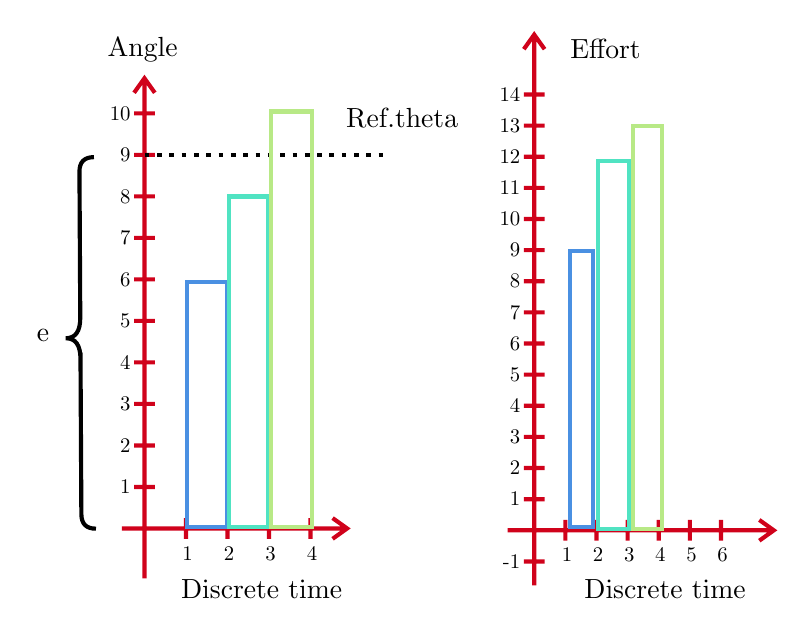
\begin{tikzpicture}[x=0.75pt,y=0.75pt,yscale=-1,xscale=1]
%uncomment if require: \path (0,530); %set diagram left start at 0, and has height of 530

%Shape: Axis 2D [id:dp6346571706526563] 
\draw [color={rgb, 255:red, 208; green, 2; blue, 27 }  ,draw opacity=1 ][line width=1.5]  (86,259.9) -- (194.5,259.9)(96.85,43) -- (96.85,284) (187.5,254.9) -- (194.5,259.9) -- (187.5,264.9) (91.85,50) -- (96.85,43) -- (101.85,50) (116.85,254.9) -- (116.85,264.9)(136.85,254.9) -- (136.85,264.9)(156.85,254.9) -- (156.85,264.9)(176.85,254.9) -- (176.85,264.9)(91.85,239.9) -- (101.85,239.9)(91.85,219.9) -- (101.85,219.9)(91.85,199.9) -- (101.85,199.9)(91.85,179.9) -- (101.85,179.9)(91.85,159.9) -- (101.85,159.9)(91.85,139.9) -- (101.85,139.9)(91.85,119.9) -- (101.85,119.9)(91.85,99.9) -- (101.85,99.9)(91.85,79.9) -- (101.85,79.9)(91.85,59.9) -- (101.85,59.9) ;
\draw   (123.85,271.9) node[anchor=east, scale=0.75]{1} (143.85,271.9) node[anchor=east, scale=0.75]{2} (163.85,271.9) node[anchor=east, scale=0.75]{3} (183.85,271.9) node[anchor=east, scale=0.75]{4} (93.85,239.9) node[anchor=east, scale=0.75]{1} (93.85,219.9) node[anchor=east, scale=0.75]{2} (93.85,199.9) node[anchor=east, scale=0.75]{3} (93.85,179.9) node[anchor=east, scale=0.75]{4} (93.85,159.9) node[anchor=east, scale=0.75]{5} (93.85,139.9) node[anchor=east, scale=0.75]{6} (93.85,119.9) node[anchor=east, scale=0.75]{7} (93.85,99.9) node[anchor=east, scale=0.75]{8} (93.85,79.9) node[anchor=east, scale=0.75]{9} (93.85,59.9) node[anchor=east, scale=0.75]{10} ;
%Straight Lines [id:da8395435041805068] 
\draw [line width=1.5]  [dash pattern={on 1.69pt off 2.76pt}]  (97,80) -- (214.5,80) ;


%Shape: Brace [id:dp15804314182279944] 
\draw  [line width=1.5]  (72.5,81) .. controls (67.83,81.03) and (65.51,83.37) .. (65.54,88.04) -- (65.93,158.23) .. controls (65.97,164.9) and (63.66,168.24) .. (58.99,168.27) .. controls (63.66,168.24) and (66.01,171.56) .. (66.04,178.23)(66.03,175.23) -- (66.46,253.04) .. controls (66.49,257.71) and (68.83,260.03) .. (73.5,260) ;
%Shape: Rectangle [id:dp5191693992255162] 
\draw  [color={rgb, 255:red, 74; green, 144; blue, 226 }  ,draw opacity=1 ][line width=1.5]  (117.5,141) -- (136.5,141) -- (136.5,259) -- (117.5,259) -- cycle ;
%Shape: Rectangle [id:dp2287664558829514] 
\draw  [color={rgb, 255:red, 80; green, 227; blue, 194 }  ,draw opacity=1 ][line width=1.5]  (137.67,100) -- (156.5,100) -- (156.5,259) -- (137.67,259) -- cycle ;
%Shape: Rectangle [id:dp3261576138135398] 
\draw  [color={rgb, 255:red, 184; green, 233; blue, 134 }  ,draw opacity=1 ][line width=1.5]  (157.67,59) -- (177.67,59) -- (177.67,259) -- (157.67,259) -- cycle ;
%Shape: Axis 2D [id:dp473563119637739] 
\draw [color={rgb, 255:red, 208; green, 2; blue, 27 }  ,draw opacity=1 ][line width=1.5]  (271.82,260.8) -- (400.08,260.8)(284.64,22) -- (284.64,287.33) (393.08,255.8) -- (400.08,260.8) -- (393.08,265.8) (279.64,29) -- (284.64,22) -- (289.64,29) (299.64,255.8) -- (299.64,265.8)(314.64,255.8) -- (314.64,265.8)(329.64,255.8) -- (329.64,265.8)(344.64,255.8) -- (344.64,265.8)(359.64,255.8) -- (359.64,265.8)(374.64,255.8) -- (374.64,265.8)(279.64,245.8) -- (289.64,245.8)(279.64,230.8) -- (289.64,230.8)(279.64,215.8) -- (289.64,215.8)(279.64,200.8) -- (289.64,200.8)(279.64,185.8) -- (289.64,185.8)(279.64,170.8) -- (289.64,170.8)(279.64,155.8) -- (289.64,155.8)(279.64,140.8) -- (289.64,140.8)(279.64,125.8) -- (289.64,125.8)(279.64,110.8) -- (289.64,110.8)(279.64,95.8) -- (289.64,95.8)(279.64,80.8) -- (289.64,80.8)(279.64,65.8) -- (289.64,65.8)(279.64,50.8) -- (289.64,50.8)(279.64,275.8) -- (289.64,275.8) ;
\draw   (306.64,272.8) node[anchor=east, scale=0.75]{1} (321.64,272.8) node[anchor=east, scale=0.75]{2} (336.64,272.8) node[anchor=east, scale=0.75]{3} (351.64,272.8) node[anchor=east, scale=0.75]{4} (366.64,272.8) node[anchor=east, scale=0.75]{5} (381.64,272.8) node[anchor=east, scale=0.75]{6} (281.64,245.8) node[anchor=east, scale=0.75]{1} (281.64,230.8) node[anchor=east, scale=0.75]{2} (281.64,215.8) node[anchor=east, scale=0.75]{3} (281.64,200.8) node[anchor=east, scale=0.75]{4} (281.64,185.8) node[anchor=east, scale=0.75]{5} (281.64,170.8) node[anchor=east, scale=0.75]{6} (281.64,155.8) node[anchor=east, scale=0.75]{7} (281.64,140.8) node[anchor=east, scale=0.75]{8} (281.64,125.8) node[anchor=east, scale=0.75]{9} (281.64,110.8) node[anchor=east, scale=0.75]{10} (281.64,95.8) node[anchor=east, scale=0.75]{11} (281.64,80.8) node[anchor=east, scale=0.75]{12} (281.64,65.8) node[anchor=east, scale=0.75]{13} (281.64,50.8) node[anchor=east, scale=0.75]{14} (281.64,275.8) node[anchor=east, scale=0.75]{-1} ;
%Shape: Rectangle [id:dp06820965849131166] 
\draw  [color={rgb, 255:red, 74; green, 144; blue, 226 }  ,draw opacity=1 ][line width=1.5]  (301.75,126.33) -- (313.08,126.33) -- (313.08,259) -- (301.75,259) -- cycle ;
%Shape: Rectangle [id:dp16997023555555235] 
\draw  [color={rgb, 255:red, 80; green, 227; blue, 194 }  ,draw opacity=1 ][line width=1.5]  (315.5,82.67) -- (330.5,82.67) -- (330.5,260) -- (315.5,260) -- cycle ;
%Shape: Rectangle [id:dp21980087841289575] 
\draw  [color={rgb, 255:red, 184; green, 233; blue, 134 }  ,draw opacity=1 ][line width=1.5]  (332.08,66) -- (346.08,66) -- (346.08,260) -- (332.08,260) -- cycle ;

% Text Node
\draw (221,62.33) node  [align=left] {Ref.theta};
% Text Node
\draw (48,167) node  [align=left] {e};
% Text Node
\draw (96,29) node  [align=left] {Angle};
% Text Node
\draw (153.33,289) node  [align=left] {Discrete time};
% Text Node
\draw (319,29) node  [align=left] {Effort};
% Text Node
\draw (347.67,289.33) node  [align=left] {Discrete time};


\end{tikzpicture}
    \caption{If the gain$K_I$ is 1 then only the sum of changes in the error has an effect on the effort.}
    \label{fig:IGain}
\end{figure}
\paragraph{The derivative} gain $K_D$ in eq. \ref{PID} of the controller, works on the rate of change in the system. So if there are a fast change when the manipulator moves or get pushed it will have a larger output in the effort within the system, but when there is no change in the system, it has no effect. This can be useful when there is a need for fast reaction within the system, but in the case of a human with a robotic prosthesis if the $K_P$ gain is too high it can result in unforeseen consequences .\\ 
\begin{figure}[H]
    \centering
    \includegraphics[width=\textwidth]{Figures/Technical_figures/DGAIN.png} 
   %

\tikzset{every picture/.style={line width=0.75pt}} %set default line width to 0.75pt        

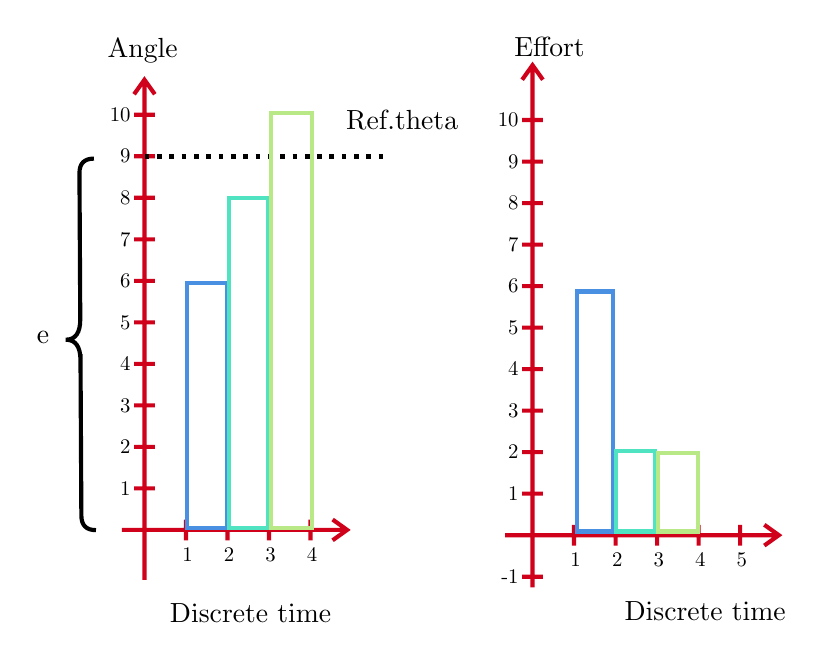
\begin{tikzpicture}[x=0.75pt,y=0.75pt,yscale=-1,xscale=1]
%uncomment if require: \path (0,530); %set diagram left start at 0, and has height of 530

%Shape: Axis 2D [id:dp9137510297707208] 
\draw [color={rgb, 255:red, 208; green, 2; blue, 27 }  ,draw opacity=1 ][line width=1.5]  (90,242.9) -- (198.5,242.9)(100.85,26) -- (100.85,267) (191.5,237.9) -- (198.5,242.9) -- (191.5,247.9) (95.85,33) -- (100.85,26) -- (105.85,33) (120.85,237.9) -- (120.85,247.9)(140.85,237.9) -- (140.85,247.9)(160.85,237.9) -- (160.85,247.9)(180.85,237.9) -- (180.85,247.9)(95.85,222.9) -- (105.85,222.9)(95.85,202.9) -- (105.85,202.9)(95.85,182.9) -- (105.85,182.9)(95.85,162.9) -- (105.85,162.9)(95.85,142.9) -- (105.85,142.9)(95.85,122.9) -- (105.85,122.9)(95.85,102.9) -- (105.85,102.9)(95.85,82.9) -- (105.85,82.9)(95.85,62.9) -- (105.85,62.9)(95.85,42.9) -- (105.85,42.9) ;
\draw   (127.85,254.9) node[anchor=east, scale=0.75]{1} (147.85,254.9) node[anchor=east, scale=0.75]{2} (167.85,254.9) node[anchor=east, scale=0.75]{3} (187.85,254.9) node[anchor=east, scale=0.75]{4} (97.85,222.9) node[anchor=east, scale=0.75]{1} (97.85,202.9) node[anchor=east, scale=0.75]{2} (97.85,182.9) node[anchor=east, scale=0.75]{3} (97.85,162.9) node[anchor=east, scale=0.75]{4} (97.85,142.9) node[anchor=east, scale=0.75]{5} (97.85,122.9) node[anchor=east, scale=0.75]{6} (97.85,102.9) node[anchor=east, scale=0.75]{7} (97.85,82.9) node[anchor=east, scale=0.75]{8} (97.85,62.9) node[anchor=east, scale=0.75]{9} (97.85,42.9) node[anchor=east, scale=0.75]{10} ;
%Straight Lines [id:da4351106715512081] 
\draw [line width=1.5]  [dash pattern={on 1.69pt off 2.76pt}]  (101,63) -- (218.5,63) ;


%Shape: Brace [id:dp994707289933978] 
\draw  [line width=1.5]  (76.5,64) .. controls (71.83,64.03) and (69.51,66.37) .. (69.54,71.04) -- (69.93,141.23) .. controls (69.97,147.9) and (67.66,151.24) .. (62.99,151.27) .. controls (67.66,151.24) and (70.01,154.56) .. (70.04,161.23)(70.03,158.23) -- (70.46,236.04) .. controls (70.49,240.71) and (72.83,243.03) .. (77.5,243) ;
%Shape: Rectangle [id:dp26090470643958286] 
\draw  [color={rgb, 255:red, 74; green, 144; blue, 226 }  ,draw opacity=1 ][line width=1.5]  (121.5,124) -- (140.5,124) -- (140.5,242) -- (121.5,242) -- cycle ;
%Shape: Rectangle [id:dp02841982011085853] 
\draw  [color={rgb, 255:red, 80; green, 227; blue, 194 }  ,draw opacity=1 ][line width=1.5]  (141.67,83) -- (160.5,83) -- (160.5,242) -- (141.67,242) -- cycle ;
%Shape: Rectangle [id:dp8528888145708966] 
\draw  [color={rgb, 255:red, 184; green, 233; blue, 134 }  ,draw opacity=1 ][line width=1.5]  (161.67,42) -- (181.67,42) -- (181.67,242) -- (161.67,242) -- cycle ;
%Shape: Axis 2D [id:dp5326952598948764] 
\draw [color={rgb, 255:red, 208; green, 2; blue, 27 }  ,draw opacity=1 ][line width=1.5]  (274.65,245.44) -- (406.5,245.44)(287.83,19) -- (287.83,270.6) (399.5,240.44) -- (406.5,245.44) -- (399.5,250.44) (282.83,26) -- (287.83,19) -- (292.83,26) (307.83,240.44) -- (307.83,250.44)(327.84,240.44) -- (327.84,250.44)(347.84,240.44) -- (347.84,250.44)(367.84,240.44) -- (367.84,250.44)(387.84,240.44) -- (387.84,250.44)(282.83,225.44) -- (292.83,225.44)(282.83,205.44) -- (292.83,205.44)(282.83,185.44) -- (292.83,185.44)(282.83,165.44) -- (292.83,165.44)(282.83,145.44) -- (292.83,145.44)(282.83,125.44) -- (292.83,125.44)(282.83,105.44) -- (292.83,105.44)(282.83,85.44) -- (292.83,85.44)(282.83,65.44) -- (292.83,65.44)(282.83,45.44) -- (292.83,45.44)(282.83,265.44) -- (292.83,265.44) ;
\draw   (314.83,257.44) node[anchor=east, scale=0.75]{1} (334.84,257.44) node[anchor=east, scale=0.75]{2} (354.84,257.44) node[anchor=east, scale=0.75]{3} (374.84,257.44) node[anchor=east, scale=0.75]{4} (394.84,257.44) node[anchor=east, scale=0.75]{5} (284.83,225.44) node[anchor=east, scale=0.75]{1} (284.83,205.44) node[anchor=east, scale=0.75]{2} (284.83,185.44) node[anchor=east, scale=0.75]{3} (284.83,165.44) node[anchor=east, scale=0.75]{4} (284.83,145.44) node[anchor=east, scale=0.75]{5} (284.83,125.44) node[anchor=east, scale=0.75]{6} (284.83,105.44) node[anchor=east, scale=0.75]{7} (284.83,85.44) node[anchor=east, scale=0.75]{8} (284.83,65.44) node[anchor=east, scale=0.75]{9} (284.83,45.44) node[anchor=east, scale=0.75]{10} (284.83,265.44) node[anchor=east, scale=0.75]{-1} ;
%Shape: Rectangle [id:dp37091810601651853] 
\draw  [color={rgb, 255:red, 74; green, 144; blue, 226 }  ,draw opacity=1 ][line width=1.5]  (309.42,128) -- (326.5,128) -- (326.5,243.67) -- (309.42,243.67) -- cycle ;
%Shape: Rectangle [id:dp5213748938493563] 
\draw  [color={rgb, 255:red, 80; green, 227; blue, 194 }  ,draw opacity=1 ][line width=1.5]  (328.08,205) -- (346.75,205) -- (346.75,243.67) -- (328.08,243.67) -- cycle ;
%Shape: Rectangle [id:dp3862836064219044] 
\draw  [color={rgb, 255:red, 184; green, 233; blue, 134 }  ,draw opacity=1 ][line width=1.5]  (348.08,206) -- (367.42,206) -- (367.42,243.67) -- (348.08,243.67) -- cycle ;

% Text Node
\draw (225,45.33) node  [align=left] {Ref.theta};
% Text Node
\draw (52,150) node  [align=left] {e};
% Text Node
\draw (100,12) node  [align=left] {Angle};
% Text Node
\draw (152,283) node  [align=left] {Discrete time};
% Text Node
\draw (296,10) node  [align=left] {Effort};
% Text Node
\draw (371,282) node  [align=left] {Discrete time};


\end{tikzpicture}
    \caption{If the gain $K_D$ is 1 then only the rate of change in the error has and effect on the effort.}
    \label{fig:DGain}
\end{figure}


\subsection*{Summery}
This project fits the EMG sensors, with electrodes on a wired connection, and an IMU onto a measuring box. This box must be connected wirelessly with radio modules to the manipulator, and be operated with low power to ensure that electrocution is not possible. The data from the measuring unit must go into a micro-controller or a pc where it is processed, and a control scheme is created and sent to the robot manipulator. 

\begin{figure}[H]
    \centering
    
\tikzset{every picture/.style={line width=0.75pt}} %set default line width to 0.75pt        

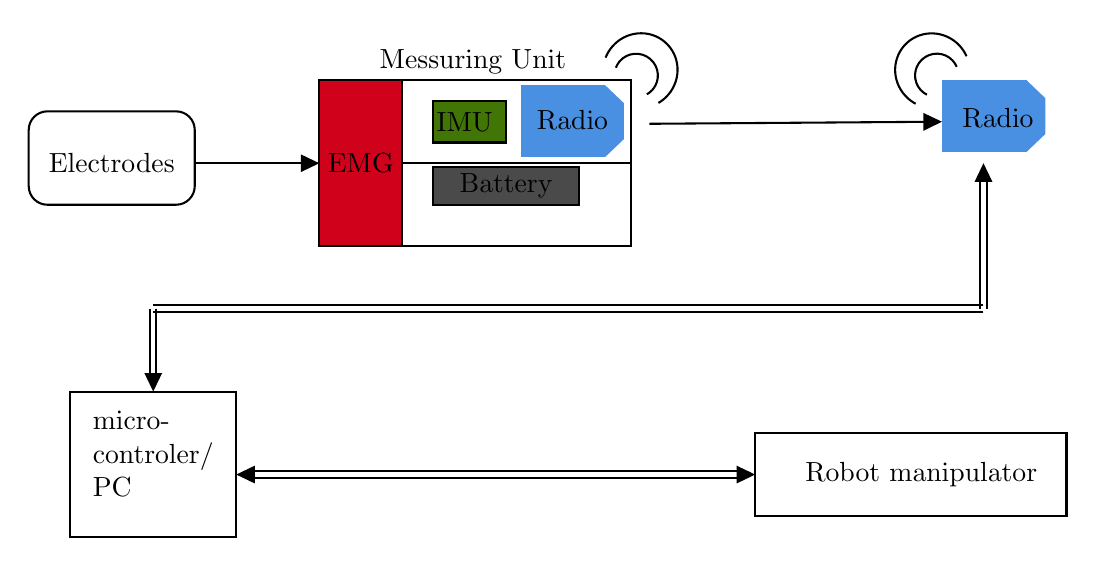
\begin{tikzpicture}[x=0.75pt,y=0.75pt,yscale=-1,xscale=1]
%uncomment if require: \path (0,278.7142848968506); %set diagram left start at 0, and has height of 278.7142848968506

%Rounded Rect [id:dp6413063332380855] 
\draw   (20,54) .. controls (20,49.03) and (24.03,45) .. (29,45) -- (91,45) .. controls (95.97,45) and (100,49.03) .. (100,54) -- (100,81) .. controls (100,85.97) and (95.97,90) .. (91,90) -- (29,90) .. controls (24.03,90) and (20,85.97) .. (20,81) -- cycle ;
%Straight Lines [id:da6300227835642365] 
\draw    (100,70) -- (158,70) ;
\draw [shift={(160,70)}, rotate = 540] [fill={rgb, 255:red, 0; green, 0; blue, 0 }  ][line width=0.75]  [draw opacity=0] (8.93,-4.29) -- (0,0) -- (8.93,4.29) -- cycle    ;

%Shape: Rectangle [id:dp29756334080248226] 
\draw   (160,30) -- (310,30) -- (310,110) -- (160,110) -- cycle ;
%Shape: Rectangle [id:dp330906364121774] 
\draw  [fill={rgb, 255:red, 208; green, 2; blue, 27 }  ,fill opacity=1 ] (160,30) -- (200,30) -- (200,110) -- (160,110) -- cycle ;
%Straight Lines [id:da029037017732416848] 
\draw    (319,51) -- (458,50.01) ;
\draw [shift={(460,50)}, rotate = 539.5899999999999] [fill={rgb, 255:red, 0; green, 0; blue, 0 }  ][line width=0.75]  [draw opacity=0] (8.93,-4.29) -- (0,0) -- (8.93,4.29) -- cycle    ;

%Shape: Rectangle [id:dp532013176046509] 
\draw   (200,30) -- (310,30) -- (310,70) -- (200,70) -- cycle ;
%Shape: Rectangle [id:dp7726211268757011] 
\draw   (200,70) -- (310,70) -- (310,110) -- (200,110) -- cycle ;
%Shape: Diagonal Stripe [id:dp8385620342618032] 
\draw  [color={rgb, 255:red, 0; green, 0; blue, 0 }  ,draw opacity=0 ][fill={rgb, 255:red, 74; green, 144; blue, 226 }  ,fill opacity=1 ] (306.79,58.36) -- (297.73,67) -- (297.73,32.43) -- (306.79,41.07) -- cycle ;
%Shape: Rectangle [id:dp048225570012627283] 
\draw  [draw opacity=0][fill={rgb, 255:red, 74; green, 144; blue, 226 }  ,fill opacity=1 ] (257,32.43) -- (297.73,32.43) -- (297.73,67) -- (257,67) -- cycle ;

%Shape: Rectangle [id:dp24678180631621505] 
\draw  [fill={rgb, 255:red, 74; green, 74; blue, 74 }  ,fill opacity=1 ] (215,72) -- (285,72) -- (285,90) -- (215,90) -- cycle ;
%Shape: Rectangle [id:dp08589280624389195] 
\draw  [fill={rgb, 255:red, 65; green, 117; blue, 5 }  ,fill opacity=1 ] (215,40) -- (250,40) -- (250,60) -- (215,60) -- cycle ;
%Shape: Arc [id:dp5045652470541955] 
\draw  [draw opacity=0] (302.89,23.99) .. controls (303.31,22.88) and (303.92,21.82) .. (304.74,20.86) .. controls (308.48,16.5) and (315.08,16.02) .. (319.46,19.79) .. controls (323.85,23.55) and (324.37,30.14) .. (320.63,34.5) .. controls (319.81,35.46) and (318.86,36.23) .. (317.82,36.8) -- (312.69,27.68) -- cycle ; \draw   (302.89,23.99) .. controls (303.31,22.88) and (303.92,21.82) .. (304.74,20.86) .. controls (308.48,16.5) and (315.08,16.02) .. (319.46,19.79) .. controls (323.85,23.55) and (324.37,30.14) .. (320.63,34.5) .. controls (319.81,35.46) and (318.86,36.23) .. (317.82,36.8) ;
%Shape: Arc [id:dp8674617821007324] 
\draw  [draw opacity=0] (297.95,19.11) .. controls (298.69,17.23) and (299.75,15.44) .. (301.14,13.82) .. controls (307.69,6.19) and (319.05,5.19) .. (326.5,11.59) .. controls (333.96,17.98) and (334.69,29.36) .. (328.14,36.99) .. controls (326.75,38.61) and (325.14,39.94) .. (323.39,40.95) -- (314.64,25.4) -- cycle ; \draw   (297.95,19.11) .. controls (298.69,17.23) and (299.75,15.44) .. (301.14,13.82) .. controls (307.69,6.19) and (319.05,5.19) .. (326.5,11.59) .. controls (333.96,17.98) and (334.69,29.36) .. (328.14,36.99) .. controls (326.75,38.61) and (325.14,39.94) .. (323.39,40.95) ;

%Shape: Arc [id:dp6395313948687686] 
\draw  [draw opacity=0] (452.73,36.97) .. controls (451.67,36.44) and (450.68,35.71) .. (449.82,34.79) .. controls (445.9,30.59) and (446.15,23.98) .. (450.38,20.04) .. controls (454.61,16.09) and (461.21,16.3) .. (465.13,20.5) .. controls (465.99,21.42) and (466.65,22.46) .. (467.11,23.55) -- (457.48,27.65) -- cycle ; \draw   (452.73,36.97) .. controls (451.67,36.44) and (450.68,35.71) .. (449.82,34.79) .. controls (445.9,30.59) and (446.15,23.98) .. (450.38,20.04) .. controls (454.61,16.09) and (461.21,16.3) .. (465.13,20.5) .. controls (465.99,21.42) and (466.65,22.46) .. (467.11,23.55) ;
%Shape: Arc [id:dp6559945001551593] 
\draw  [draw opacity=0] (447.33,41.35) .. controls (445.55,40.4) and (443.88,39.15) .. (442.42,37.58) .. controls (435.56,30.23) and (435.82,18.84) .. (443.01,12.13) .. controls (450.19,5.43) and (461.58,5.96) .. (468.44,13.31) .. controls (469.9,14.88) and (471.03,16.63) .. (471.85,18.47) -- (455.43,25.45) -- cycle ; \draw   (447.33,41.35) .. controls (445.55,40.4) and (443.88,39.15) .. (442.42,37.58) .. controls (435.56,30.23) and (435.82,18.84) .. (443.01,12.13) .. controls (450.19,5.43) and (461.58,5.96) .. (468.44,13.31) .. controls (469.9,14.88) and (471.03,16.63) .. (471.85,18.47) ;

%Straight Lines [id:da36130723234012985] 
\draw    (481.5,78) -- (481.5,140)(478.5,78) -- (478.5,140) ;

\draw [shift={(480,70)}, rotate = 90] [fill={rgb, 255:red, 0; green, 0; blue, 0 }  ][line width=0.75]  [draw opacity=0] (8.93,-4.29) -- (0,0) -- (8.93,4.29) -- cycle    ;
%Straight Lines [id:da3368128282424796] 
\draw    (480,141.5) -- (80,141.5)(480,138.5) -- (80,138.5) ;


%Straight Lines [id:da6986678551956043] 
\draw    (81.5,140) -- (81.5,172)(78.5,140) -- (78.5,172) ;
\draw [shift={(80,180)}, rotate = 270] [fill={rgb, 255:red, 0; green, 0; blue, 0 }  ][line width=0.75]  [draw opacity=0] (8.93,-4.29) -- (0,0) -- (8.93,4.29) -- cycle    ;

%Straight Lines [id:da17642820100898704] 
\draw    (128,218.5) -- (362,218.5)(128,221.5) -- (362,221.5) ;
\draw [shift={(370,220)}, rotate = 180] [fill={rgb, 255:red, 0; green, 0; blue, 0 }  ][line width=0.75]  [draw opacity=0] (8.93,-4.29) -- (0,0) -- (8.93,4.29) -- cycle    ;
\draw [shift={(120,220)}, rotate = 0] [fill={rgb, 255:red, 0; green, 0; blue, 0 }  ][line width=0.75]  [draw opacity=0] (8.93,-4.29) -- (0,0) -- (8.93,4.29) -- cycle    ;
%Shape: Rectangle [id:dp18164367926693248] 
\draw   (370,200) -- (520,200) -- (520,240) -- (370,240) -- cycle ;
%Shape: Diagonal Stripe [id:dp43939989252487766] 
\draw  [color={rgb, 255:red, 0; green, 0; blue, 0 }  ,draw opacity=0 ][fill={rgb, 255:red, 74; green, 144; blue, 226 }  ,fill opacity=1 ] (509.79,55.93) -- (500.73,64.57) -- (500.73,30) -- (509.79,38.64) -- cycle ;
%Shape: Rectangle [id:dp8507327329990411] 
\draw  [draw opacity=0][fill={rgb, 255:red, 74; green, 144; blue, 226 }  ,fill opacity=1 ] (460,30) -- (500.73,30) -- (500.73,64.57) -- (460,64.57) -- cycle ;
%Shape: Rectangle [id:dp7178522299746128] 
\draw   (40,180) -- (120,180) -- (120,250) -- (40,250) -- cycle ;

% Text Node
\draw (60,70) node  [align=left] {Electrodes};
% Text Node
\draw (234,21) node  [align=left] {Messuring Unit};
% Text Node
\draw (282,49) node  [align=left] {Radio};
% Text Node
\draw (250,81) node  [align=left] {Battery};
% Text Node
\draw (180,70) node  [align=left] {EMG};
% Text Node
\draw (230,50) node  [align=left] {IMU};
% Text Node
\draw (450,220) node  [align=left] {Robot manipulator};
% Text Node
\draw (80,210) node  [align=left] {micro-\\controler/\\PC};
% Text Node
\draw (487,48) node  [align=left] {Radio};


\end{tikzpicture}
\caption{Illustration of the general design solution. Arrows indicates the direction information is send.}
    \label{fig:GenDesign}
\end{figure}

\section{Delimitation's}\label{Delimitations}
To design a complete prosthesis for a person with shoulder-disarticulation requires that there are money and time available to do so. Due to the lack of money and time in this project, a concept based prosthesis will be built upon the design of the CrustCrawler robotic manipulator from CrustCrawler robotics, the CrustCrawler is implemented with servos from Dynamixel. \\
The controls for the prosthesis will be limited to two sEMG signals and three signals from an accelerometer, the number of signals from the user will limit the control design approach. All these components will be described in the next chapters.\\
In order to save time, this project will not create a shoulder mounting and the placement of the robotic prosthesis is on a table, where the control system can still be created and tested.


\section{Specific design solution}
\subsection*{Equipment description}
For this project several pieces of equipment have been provided, as such this project will investigate how these components can be used to accomplish our goal. The provided equipment can be read about in the following sections.


\begin{table}[H]
\begin{tabular}{|P{3cm}||P{10cm}|}

\hline
CrustCrawler & The manipulator consisting of 5 motors \\ \hline
Motors                 & All five motors mounted on the CrustCrawler are made by Dynamixel.  \\ \hline
Xbee S1                  & Wireless radio capable of pairing to matching device creating a connection between the two Xbee modules \\ \hline
Teensy 3.5 Board              & Microcontroller that works as the on board computer.      \\ \hline
Supply  board             & Power-supply board connected to a wall plug and the system                  \\ \hline
\end{tabular}%
\caption{Description and presentation of the CrustCrawler setup components}
\label{tableCrust}
\end{table}


\begin{table}[H]
\begin{tabular}{|P{3cm}||P{10cm}|}
\hline
\textbf{Measuring box} & This system consists of several components housed in a 3D printed box   \\ \hline
XBee S1                  & Wireless radio capable of pairing to matching device creating an "instant link" \\ \hline
Battery                  & Type CR123A, normally used for cameras                                  \\ \hline
5x Inputs                & 2 x Sparkfun EMG boards + 3 axis Accelerometer                         \\ \hline
\end{tabular}%
\caption{Description of components in the measuring box}
\label{tableBOX}
\end{table}
\noindent
The figure \ref{fig:SpecificDesign} shows the data flow and the components of the solution presented in this chapter.
\begin{figure}[H]
    \centering
    

\tikzset{every picture/.style={line width=0.75pt}} %set default line width to 0.75pt        

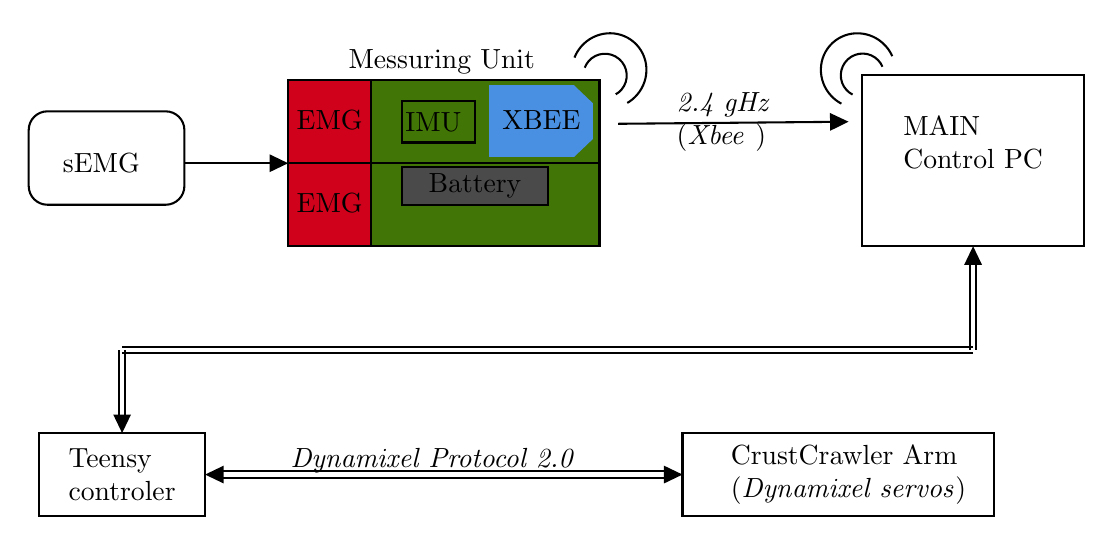
\begin{tikzpicture}[x=0.75pt,y=0.75pt,yscale=-1,xscale=1]
%uncomment if require: \path (0,278.7142848968506); %set diagram left start at 0, and has height of 278.7142848968506

%Shape: Rectangle [id:dp9058146125823148] 
\draw   (436.69,27.6) -- (543.37,27.6) -- (543.37,110) -- (436.69,110) -- cycle ;
%Rounded Rect [id:dp9198394438295476] 
\draw   (35,54) .. controls (35,49.03) and (39.03,45) .. (44,45) -- (101,45) .. controls (105.97,45) and (110,49.03) .. (110,54) -- (110,81) .. controls (110,85.97) and (105.97,90) .. (101,90) -- (44,90) .. controls (39.03,90) and (35,85.97) .. (35,81) -- cycle ;
%Straight Lines [id:da08300314610956905] 
\draw    (110,70) -- (158,70) ;
\draw [shift={(160,70)}, rotate = 180] [fill={rgb, 255:red, 0; green, 0; blue, 0 }  ][line width=0.75]  [draw opacity=0] (8.93,-4.29) -- (0,0) -- (8.93,4.29) -- cycle    ;

%Shape: Rectangle [id:dp49994760485296896] 
\draw  [fill={rgb, 255:red, 65; green, 117; blue, 5 }  ,fill opacity=1 ] (160,30) -- (310,30) -- (310,110) -- (160,110) -- cycle ;
%Shape: Rectangle [id:dp9990642544965083] 
\draw  [fill={rgb, 255:red, 208; green, 2; blue, 27 }  ,fill opacity=1 ] (160,30) -- (200,30) -- (200,70) -- (160,70) -- cycle ;
%Shape: Rectangle [id:dp5155575250253981] 
\draw  [fill={rgb, 255:red, 208; green, 2; blue, 27 }  ,fill opacity=1 ] (160,70) -- (200,70) -- (200,110) -- (160,110) -- cycle ;
%Straight Lines [id:da2266079205645528] 
\draw    (319,51) -- (428,50.02) ;
\draw [shift={(430,50)}, rotate = 539.48] [fill={rgb, 255:red, 0; green, 0; blue, 0 }  ][line width=0.75]  [draw opacity=0] (8.93,-4.29) -- (0,0) -- (8.93,4.29) -- cycle    ;

%Shape: Rectangle [id:dp7097032559017205] 
\draw  [fill={rgb, 255:red, 65; green, 117; blue, 5 }  ,fill opacity=1 ] (200,30) -- (310,30) -- (310,70) -- (200,70) -- cycle ;
%Shape: Rectangle [id:dp16739603109917534] 
\draw  [fill={rgb, 255:red, 65; green, 117; blue, 5 }  ,fill opacity=1 ] (200,70) -- (310,70) -- (310,110) -- (200,110) -- cycle ;
%Shape: Diagonal Stripe [id:dp825501516378429] 
\draw  [color={rgb, 255:red, 0; green, 0; blue, 0 }  ,draw opacity=0 ][fill={rgb, 255:red, 74; green, 144; blue, 226 }  ,fill opacity=1 ] (306.79,58.36) -- (297.73,67) -- (297.73,32.43) -- (306.79,41.07) -- cycle ;
%Shape: Rectangle [id:dp443446878421101] 
\draw  [draw opacity=0][fill={rgb, 255:red, 74; green, 144; blue, 226 }  ,fill opacity=1 ] (257,32.43) -- (297.73,32.43) -- (297.73,67) -- (257,67) -- cycle ;

%Shape: Rectangle [id:dp7890442898232035] 
\draw  [fill={rgb, 255:red, 74; green, 74; blue, 74 }  ,fill opacity=1 ] (215,72) -- (285,72) -- (285,90) -- (215,90) -- cycle ;
%Shape: Rectangle [id:dp3185767197775584] 
\draw  [fill={rgb, 255:red, 65; green, 117; blue, 5 }  ,fill opacity=1 ] (215,40) -- (250,40) -- (250,60) -- (215,60) -- cycle ;
%Shape: Arc [id:dp6014275798651711] 
\draw  [draw opacity=0] (302.89,23.99) .. controls (303.31,22.88) and (303.92,21.82) .. (304.74,20.86) .. controls (308.48,16.5) and (315.08,16.02) .. (319.46,19.79) .. controls (323.85,23.55) and (324.37,30.14) .. (320.63,34.5) .. controls (319.81,35.46) and (318.86,36.23) .. (317.82,36.8) -- (312.69,27.68) -- cycle ; \draw   (302.89,23.99) .. controls (303.31,22.88) and (303.92,21.82) .. (304.74,20.86) .. controls (308.48,16.5) and (315.08,16.02) .. (319.46,19.79) .. controls (323.85,23.55) and (324.37,30.14) .. (320.63,34.5) .. controls (319.81,35.46) and (318.86,36.23) .. (317.82,36.8) ;
%Shape: Arc [id:dp584505117797834] 
\draw  [draw opacity=0] (297.95,19.11) .. controls (298.69,17.23) and (299.75,15.44) .. (301.14,13.82) .. controls (307.69,6.19) and (319.05,5.19) .. (326.5,11.59) .. controls (333.96,17.98) and (334.69,29.36) .. (328.14,36.99) .. controls (326.75,38.61) and (325.14,39.94) .. (323.39,40.95) -- (314.64,25.4) -- cycle ; \draw   (297.95,19.11) .. controls (298.69,17.23) and (299.75,15.44) .. (301.14,13.82) .. controls (307.69,6.19) and (319.05,5.19) .. (326.5,11.59) .. controls (333.96,17.98) and (334.69,29.36) .. (328.14,36.99) .. controls (326.75,38.61) and (325.14,39.94) .. (323.39,40.95) ;

%Shape: Arc [id:dp9643215893864674] 
\draw  [draw opacity=0] (431.94,36.92) .. controls (430.88,36.39) and (429.9,35.66) .. (429.04,34.74) .. controls (425.12,30.54) and (425.37,23.93) .. (429.6,19.99) .. controls (433.82,16.04) and (440.43,16.25) .. (444.35,20.46) .. controls (445.21,21.38) and (445.87,22.41) .. (446.33,23.51) -- (436.69,27.6) -- cycle ; \draw   (431.94,36.92) .. controls (430.88,36.39) and (429.9,35.66) .. (429.04,34.74) .. controls (425.12,30.54) and (425.37,23.93) .. (429.6,19.99) .. controls (433.82,16.04) and (440.43,16.25) .. (444.35,20.46) .. controls (445.21,21.38) and (445.87,22.41) .. (446.33,23.51) ;
%Shape: Arc [id:dp6589182805450249] 
\draw  [draw opacity=0] (426.55,41.3) .. controls (424.76,40.36) and (423.1,39.1) .. (421.64,37.54) .. controls (414.78,30.18) and (415.04,18.79) .. (422.22,12.09) .. controls (429.41,5.39) and (440.79,5.91) .. (447.65,13.27) .. controls (449.11,14.83) and (450.25,16.58) .. (451.07,18.43) -- (434.64,25.4) -- cycle ; \draw   (426.55,41.3) .. controls (424.76,40.36) and (423.1,39.1) .. (421.64,37.54) .. controls (414.78,30.18) and (415.04,18.79) .. (422.22,12.09) .. controls (429.41,5.39) and (440.79,5.91) .. (447.65,13.27) .. controls (449.11,14.83) and (450.25,16.58) .. (451.07,18.43) ;

%Straight Lines [id:da8446148813559833] 
\draw    (491.5,118) -- (491.5,160)(488.5,118) -- (488.5,160) ;

\draw [shift={(490,110)}, rotate = 90] [fill={rgb, 255:red, 0; green, 0; blue, 0 }  ][line width=0.75]  [draw opacity=0] (8.93,-4.29) -- (0,0) -- (8.93,4.29) -- cycle    ;
%Straight Lines [id:da5044267925519024] 
\draw    (490,161.5) -- (80,161.5)(490,158.5) -- (80,158.5) ;


%Straight Lines [id:da7406026285596496] 
\draw    (81.5,160) -- (81.5,192)(78.5,160) -- (78.5,192) ;
\draw [shift={(80,200)}, rotate = 270] [fill={rgb, 255:red, 0; green, 0; blue, 0 }  ][line width=0.75]  [draw opacity=0] (8.93,-4.29) -- (0,0) -- (8.93,4.29) -- cycle    ;

%Shape: Rectangle [id:dp016623272212034745] 
\draw   (40,200) -- (120,200) -- (120,240) -- (40,240) -- cycle ;
%Straight Lines [id:da7263406511929] 
\draw    (128,218.5) -- (342,218.5)(128,221.5) -- (342,221.5) ;
\draw [shift={(350,220)}, rotate = 180] [fill={rgb, 255:red, 0; green, 0; blue, 0 }  ][line width=0.75]  [draw opacity=0] (8.93,-4.29) -- (0,0) -- (8.93,4.29) -- cycle    ;
\draw [shift={(120,220)}, rotate = 0] [fill={rgb, 255:red, 0; green, 0; blue, 0 }  ][line width=0.75]  [draw opacity=0] (8.93,-4.29) -- (0,0) -- (8.93,4.29) -- cycle    ;
%Shape: Rectangle [id:dp6457555540924869] 
\draw   (350,200) -- (500,200) -- (500,240) -- (350,240) -- cycle ;

% Text Node
\draw (490,60) node  [align=left] {MAIN\\Control PC};
% Text Node
\draw (70,70) node  [align=left] {sEMG};
% Text Node
\draw (234,21) node  [align=left] {Messuring Unit};
% Text Node
\draw (282,49) node  [align=left] {XBEE};
% Text Node
\draw (370,50) node  [align=left] {\textit{2.4 gHz}\\(\textit{Xbee })};
% Text Node
\draw (250,81) node  [align=left] {Battery};
% Text Node
\draw (180,49) node  [align=left] {EMG};
% Text Node
\draw (180,89) node  [align=left] {EMG};
% Text Node
\draw (230,50) node  [align=left] {IMU};
% Text Node
\draw (80,220) node  [align=left] {Teensy\\controler};
% Text Node
\draw (230,220) node  [align=left] {\textit{Dynamixel Protocol 2.0}\\};
% Text Node
\draw (430,220) node  [align=left] {CrustCrawler Arm\\(\textit{Dynamixel servos})};


\end{tikzpicture}

    \caption{Data flowchart}
    \label{fig:DataFlow}
\end{figure}
%\begin{figure}
 %   \centering
  %  \includegraphics[width=\textwidth]{Figures/Technical_figures/jk.PNG}
   % \caption{Data flowchart}
    %\label{fig:Dataflowchar}
%\end{figure}
\subsection*{Measuring box}
This box consists of two Sparkfun Muscle Sensor Platinum V3.3 EMG sensors, one Polulo 3-Axis Accelerometer, a CR123A battery and an XBee S1 radio module, which can be read about below.

\subsubsection*{EMG detection unit - Sparkfun EMG sensors}
The EMG sensor measures the difference in potential within the muscles, however, this is not what is received by the rest of the system. First, the raw potential signal is sent through a circuit that rectifies the potential. After this, a small number of data points is then summed and averaged to smooth the data out in the smooth circuit. After the rectification and smoothing the data is sent to the XBee, which is described in depth in section \ref{sec:elHW}.\\
A full schematic of the EMG sensors can be seen in Appendix \ref{app:EMGsensor}

\subsubsection*{IMU - Polulo Accelerometer}
The polulo accelerometer consists of both a gyroscope for direction sensing and an accelerometer for g-force detection. The g-force sensitivity of the polulo accelerometer goes up to 16 g's, although the g-force used in this project is around +/- 2g. Hereby it is concluded that both accelerometer and gyroscope is available, and only a small amount of g-force can decide the direction of choice \cite{Acceleration}.

\subsubsection*{Radio module - Xbee S1}\label{XbeeExplan}
The XBee S1 radio module is the foundation of the wireless transmission of data in this solution. It has a frequency of $100Hz$ and sends a frame on every sample which is created every $0.10s$, the frame consists of 24 bytes. The structure of the 24 bytes can be seen below in figure \ref{fig:XbeeFrame}
\begin{figure}[H]
    \centering
    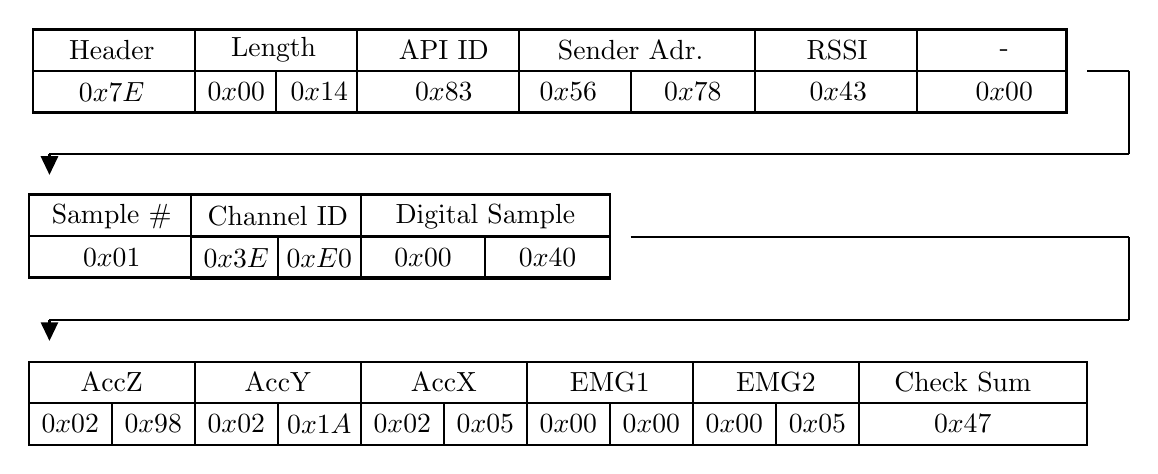
\begin{tikzpicture}[x=0.75pt,y=0.75pt,yscale=-1,xscale=1]
%uncomment if require: \path (0,230.14285278320312); %set diagram left start at 0, and has height of 230.14285278320312

%Shape: Rectangle [id:dp10856467985503815] 
\draw   (22,10) -- (520,10) -- (520,50) -- (22,50) -- cycle ;
%Shape: Rectangle [id:dp1921303622580388] 
\draw   (22,10) -- (100,10) -- (100,30) -- (22,30) -- cycle ;
%Shape: Rectangle [id:dp5511536446299157] 
\draw   (22,30) -- (100,30) -- (100,50) -- (22,50) -- cycle ;
%Shape: Rectangle [id:dp8551124842169571] 
\draw   (100,30) -- (178,30) -- (178,50) -- (100,50) -- cycle ;
%Shape: Rectangle [id:dp1542301721460031] 
\draw   (100,10) -- (178,10) -- (178,30) -- (100,30) -- cycle ;
%Shape: Rectangle [id:dp39637490877675896] 
\draw   (100,30) -- (139,30) -- (139,50) -- (100,50) -- cycle ;
%Shape: Rectangle [id:dp7008641367286479] 
\draw   (178,10) -- (256,10) -- (256,30) -- (178,30) -- cycle ;
%Shape: Rectangle [id:dp6311822380704302] 
\draw   (178,30) -- (256,30) -- (256,50) -- (178,50) -- cycle ;
%Shape: Rectangle [id:dp2794130706147937] 
\draw   (256,10) -- (370,10) -- (370,30) -- (256,30) -- cycle ;
%Shape: Rectangle [id:dp0748834298647747] 
\draw   (256,30) -- (370,30) -- (370,50) -- (256,50) -- cycle ;
%Shape: Rectangle [id:dp3442757233060003] 
\draw   (256,30) -- (310,30) -- (310,50) -- (256,50) -- cycle ;
%Shape: Rectangle [id:dp7243088972581471] 
\draw   (370,10) -- (448,10) -- (448,30) -- (370,30) -- cycle ;
%Shape: Rectangle [id:dp8634226198686377] 
\draw   (370,30) -- (448,30) -- (448,50) -- (370,50) -- cycle ;
%Shape: Rectangle [id:dp049451176775102246] 
\draw   (448,30) -- (520,30) -- (520,50) -- (448,50) -- cycle ;
%Shape: Rectangle [id:dp10185955763756471] 
\draw   (448,10) -- (520,10) -- (520,30) -- (448,30) -- cycle ;
%Shape: Rectangle [id:dp3116685664620873] 
\draw   (20,89.5) -- (300,89.5) -- (300,129.5) -- (20,129.5) -- cycle ;
%Shape: Rectangle [id:dp4024383934360989] 
\draw   (20,89.5) -- (98,89.5) -- (98,109.5) -- (20,109.5) -- cycle ;
%Shape: Rectangle [id:dp9664793454969085] 
\draw   (20,109.5) -- (98,109.5) -- (98,129.5) -- (20,129.5) -- cycle ;
%Shape: Rectangle [id:dp4124508293977984] 
\draw   (98,109.5) -- (180,109.5) -- (180,129.5) -- (98,129.5) -- cycle ;
%Shape: Rectangle [id:dp711781414287457] 
\draw   (98,89.5) -- (180,89.5) -- (180,110) -- (98,110) -- cycle ;
%Shape: Rectangle [id:dp356328253424953] 
\draw   (98,110) -- (140,110) -- (140,130) -- (98,130) -- cycle ;
%Shape: Rectangle [id:dp6733077815498894] 
\draw   (180,89.5) -- (300,89.5) -- (300,110) -- (180,110) -- cycle ;
%Shape: Rectangle [id:dp6479637887159722] 
\draw   (180,109.5) -- (300,109.5) -- (300,130) -- (180,130) -- cycle ;
%Shape: Rectangle [id:dp19346515996870206] 
\draw   (180,110) -- (240,110) -- (240,130) -- (180,130) -- cycle ;
%Shape: Rectangle [id:dp38146177317207886] 
\draw   (20,170) -- (530,170) -- (530,210) -- (20,210) -- cycle ;
%Shape: Rectangle [id:dp4556101293933754] 
\draw   (20,170) -- (100,170) -- (100,190) -- (20,190) -- cycle ;
%Shape: Rectangle [id:dp5407175554825892] 
\draw   (20,190) -- (60,190) -- (60,210) -- (20,210) -- cycle ;
%Shape: Rectangle [id:dp7450461679704352] 
\draw   (60,190) -- (100,190) -- (100,210) -- (60,210) -- cycle ;
%Shape: Rectangle [id:dp4332754864269053] 
\draw   (100,170) -- (180,170) -- (180,190) -- (100,190) -- cycle ;
%Shape: Rectangle [id:dp28452698286293754] 
\draw   (140,190) -- (180,190) -- (180,210) -- (140,210) -- cycle ;
%Shape: Rectangle [id:dp7914115317030024] 
\draw   (100,190) -- (140,190) -- (140,210) -- (100,210) -- cycle ;
%Shape: Rectangle [id:dp38727788354631554] 
\draw   (220,190) -- (260,190) -- (260,210) -- (220,210) -- cycle ;
%Shape: Rectangle [id:dp22288528455712386] 
\draw   (180,190) -- (220,190) -- (220,210) -- (180,210) -- cycle ;
%Shape: Rectangle [id:dp8165391393896375] 
\draw   (180,170) -- (260,170) -- (260,190) -- (180,190) -- cycle ;
%Shape: Rectangle [id:dp6523955550843537] 
\draw   (260,190) -- (300,190) -- (300,210) -- (260,210) -- cycle ;
%Shape: Rectangle [id:dp9747757771531758] 
\draw   (300,190) -- (340,190) -- (340,210) -- (300,210) -- cycle ;
%Shape: Rectangle [id:dp8745951425419776] 
\draw   (260,170) -- (340,170) -- (340,190) -- (260,190) -- cycle ;
%Shape: Rectangle [id:dp9793885365492223] 
\draw   (340,170) -- (420,170) -- (420,190) -- (340,190) -- cycle ;
%Shape: Rectangle [id:dp03157812028724449] 
\draw   (340,190) -- (380,190) -- (380,210) -- (340,210) -- cycle ;
%Shape: Rectangle [id:dp24057366681022452] 
\draw   (380,190) -- (420,190) -- (420,210) -- (380,210) -- cycle ;
%Shape: Rectangle [id:dp36093082441092617] 
\draw   (140,110) -- (180,110) -- (180,130) -- (140,130) -- cycle ;
%Shape: Rectangle [id:dp7171363093153074] 
\draw   (420,170) -- (530,170) -- (530,190) -- (420,190) -- cycle ;
%Shape: Rectangle [id:dp5647098232631986] 
\draw   (420,190) -- (530,190) -- (530,210) -- (420,210) -- cycle ;
%Straight Lines [id:da6332689457085323] 
\draw    (530,30) -- (550,30) ;


%Straight Lines [id:da30561509563968503] 
\draw    (550,30) -- (550,70) ;


%Straight Lines [id:da09566559311573841] 
\draw    (550,70) -- (30,70) ;


%Straight Lines [id:da5601518731242143] 
\draw    (30,70) -- (30,78) ;
\draw [shift={(30,80)}, rotate = 270] [fill={rgb, 255:red, 0; green, 0; blue, 0 }  ][line width=0.75]  [draw opacity=0] (8.93,-4.29) -- (0,0) -- (8.93,4.29) -- cycle    ;

%Straight Lines [id:da9169109459317539] 
\draw    (310,110) -- (550,110) ;


%Straight Lines [id:da5912944234587121] 
\draw    (550,110) -- (550,150) ;


%Straight Lines [id:da7375405804531086] 
\draw    (550,150) -- (30,150) ;


%Straight Lines [id:da024754719673693026] 
\draw    (30,150) -- (30,158) ;
\draw [shift={(30,160)}, rotate = 270] [fill={rgb, 255:red, 0; green, 0; blue, 0 }  ][line width=0.75]  [draw opacity=0] (8.93,-4.29) -- (0,0) -- (8.93,4.29) -- cycle    ;


% Text Node
\draw (60,20) node  [align=left] {Header};
% Text Node
\draw (60,40) node   {$0x7E$};
% Text Node
\draw (138,19.5) node  [align=left] {Length};
% Text Node
\draw (120,40) node   {$0x00$};
% Text Node
\draw (160,40) node   {$0x14$};
% Text Node
\draw (220,20) node  [align=left] {API ID};
% Text Node
\draw (220,40) node   {$0x83$};
% Text Node
\draw (310,20) node  [align=left] {Sender Adr.};
% Text Node
\draw (280,40) node   {$0x56$};
% Text Node
\draw (340,40) node   {$0x78$};
% Text Node
\draw (409.5,20) node  [align=left] {RSSI};
% Text Node
\draw (410,40) node   {$0x43$};
% Text Node
\draw (490,20) node  [align=left] {\mbox{-}};
% Text Node
\draw (490,40) node   {$0x00$};
% Text Node
\draw (60,100) node  [align=left] {Sample \#};
% Text Node
\draw (60,120) node   {$0x01$};
% Text Node
\draw (140,100) node  [align=left] {Channel ID};
% Text Node
\draw (120,120) node   {$0x3E$};
% Text Node
\draw (160,120) node   {$0xE0$};
% Text Node
\draw (240,100) node  [align=left] {Digital Sample};
% Text Node
\draw (210,120) node   {$0x00$};
% Text Node
\draw (270,120) node   {$0x40$};
% Text Node
\draw (60,180) node  [align=left] {AccZ};
% Text Node
\draw (40,200) node   {$0x02$};
% Text Node
\draw (80,200) node   {$0x98$};
% Text Node
\draw (140,180) node  [align=left] {AccY};
% Text Node
\draw (120,200) node   {$0x02$};
% Text Node
\draw (160,200) node   {$0x1A$};
% Text Node
\draw (220,180) node  [align=left] {AccX};
% Text Node
\draw (200,200) node   {$0x02$};
% Text Node
\draw (240,200) node   {$0x05$};
% Text Node
\draw (280,200) node   {$0x00$};
% Text Node
\draw (320,200) node   {$0x00$};
% Text Node
\draw (300,180) node  [align=left] {EMG1};
% Text Node
\draw (360,200) node   {$0x00$};
% Text Node
\draw (400,200) node   {$0x05$};
% Text Node
\draw (380,180) node  [align=left] {EMG2};
% Text Node
\draw (470,180) node  [align=left] {Check Sum};
% Text Node
\draw (470,200) node   {$0x47$};


\end{tikzpicture}

    \caption{XBee Frame arrows indicate the direction to read.}
    \label{fig:XbeeFrame}
\end{figure}\label{XbeeDataStruct}
The first is the header-byte that determines the start of a new frame, after the header-byte there is the length information of the frame that checks if all 24 bytes are in the frame. Afterwards, there is information on the XBee module followed by data gathered from the sensors and is ended by the CheckSum that checks if the data is transferred correctly.
\subsection*{Microcontroller - Teensy 3.5}
The small 62.4 mm x 18.0 mm teensy 3.5 micro-controller, has many features implemented, such as a 32-bit 120MHz processor capable of accessing several ADCs (Analog to digital converters). This feature is useful as it can convert analog voltage on a pin to a digital number. Furthermore these digital pins have interrupt capability and are 5 volt tolerant.\\
The micro controller is build with a micro SD card slot which is capable of storing projects up to 512 kilobytes and a Electrically Erasable Programmable Read-Only-Memory(EEPROM), that can erase data by adding a electrical charge, much like a flash-memory, only that EEPROM keeps the data until the electric charge is added.\\
The Teensy receives the information from the measuring box and the robot. The measuring unit data is converted into an output that is readable to the robot \cite{Teensy1}.

\subsubsection*{RS232 to RS485} \label{sec:RS485}
The radio module and robot runs with two different communication standards. Therefore a conversion unit between the two standards is needed,this project uses the BOB-10124 to handle the conversion. 
\begin{figure}[H]
    \centering
    

\tikzset{every picture/.style={line width=0.75pt}} %set default line width to 0.75pt        

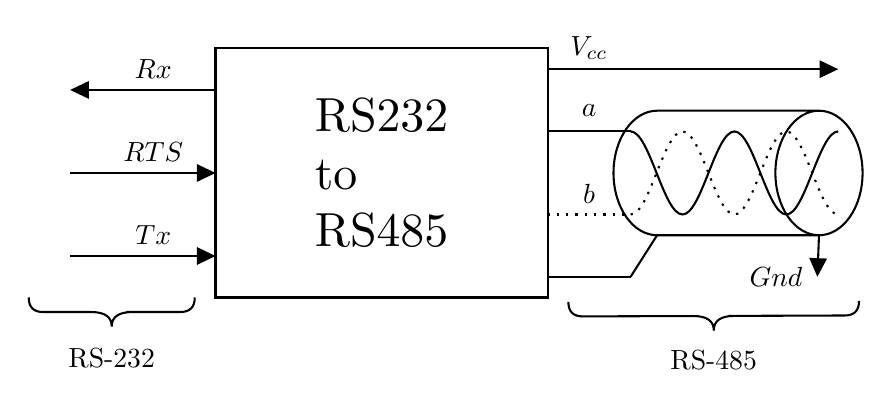
\begin{tikzpicture}[x=0.75pt,y=0.75pt,yscale=-1,xscale=1]
%uncomment if require: \path (0,217.6363525390625); %set diagram left start at 0, and has height of 217.6363525390625

%Shape: Rectangle [id:dp992532621229332] 
\draw   (100,30) -- (260,30) -- (260,150) -- (100,150) -- cycle ;
%Straight Lines [id:da5747180744657265] 
\draw    (32,50) -- (100,50) ;

\draw [shift={(30,50)}, rotate = 0] [fill={rgb, 255:red, 0; green, 0; blue, 0 }  ][line width=0.75]  [draw opacity=0] (8.93,-4.29) -- (0,0) -- (8.93,4.29) -- cycle    ;
%Straight Lines [id:da22964301218996663] 
\draw    (30,90) -- (98,90) ;
\draw [shift={(100,90)}, rotate = 180] [fill={rgb, 255:red, 0; green, 0; blue, 0 }  ][line width=0.75]  [draw opacity=0] (8.93,-4.29) -- (0,0) -- (8.93,4.29) -- cycle    ;

%Straight Lines [id:da2677261187564559] 
\draw    (30,130) -- (98,130) ;
\draw [shift={(100,130)}, rotate = 180] [fill={rgb, 255:red, 0; green, 0; blue, 0 }  ][line width=0.75]  [draw opacity=0] (8.93,-4.29) -- (0,0) -- (8.93,4.29) -- cycle    ;

%Straight Lines [id:da5541489716106782] 
\draw  [dash pattern={on 0.84pt off 2.51pt}]  (260,110) -- (300,110) ;


%Straight Lines [id:da09956683895016183] 
\draw    (260,70) -- (300,70) ;


%Shape: Wave [id:dp6378387303335409] 
\draw  [dash pattern={on 0.84pt off 2.51pt}] (300,110) .. controls (304.52,110) and (308.42,100.25) .. (312.5,90) .. controls (316.58,79.75) and (320.48,70) .. (325,70) .. controls (329.52,70) and (333.42,79.75) .. (337.5,90) .. controls (341.58,100.25) and (345.48,110) .. (350,110) .. controls (354.52,110) and (358.42,100.25) .. (362.5,90) .. controls (366.58,79.75) and (370.48,70) .. (375,70) .. controls (379.52,70) and (383.42,79.75) .. (387.5,90) .. controls (391.58,100.25) and (395.48,110) .. (400,110) ;
%Shape: Wave [id:dp12967964362630724] 
\draw   (300,70) .. controls (304.52,70) and (308.42,79.75) .. (312.5,90) .. controls (316.58,100.25) and (320.48,110) .. (325,110) .. controls (329.52,110) and (333.42,100.25) .. (337.5,90) .. controls (341.58,79.75) and (345.48,70) .. (350,70) .. controls (354.52,70) and (358.42,79.75) .. (362.5,90) .. controls (366.58,100.25) and (370.48,110) .. (375,110) .. controls (379.52,110) and (383.42,100.25) .. (387.5,90) .. controls (391.58,79.75) and (395.48,70) .. (400,70) ;
%Straight Lines [id:da2654543253939561] 
\draw    (260,140) -- (300,140) ;


%Flowchart: Direct Access Storage [id:dp6439756816416224] 
\draw   (390.75,120) -- (312.75,120) .. controls (301.15,120) and (291.75,106.57) .. (291.75,90) .. controls (291.75,73.43) and (301.15,60) .. (312.75,60) -- (390.75,60)(411.75,90) .. controls (411.75,106.57) and (402.35,120) .. (390.75,120) .. controls (379.15,120) and (369.75,106.57) .. (369.75,90) .. controls (369.75,73.43) and (379.15,60) .. (390.75,60) .. controls (402.35,60) and (411.75,73.43) .. (411.75,90) ;
%Straight Lines [id:da25800191363461744] 
\draw    (300,140) -- (312.75,120) ;


%Straight Lines [id:da7111201241992133] 
\draw    (390.75,120) -- (390.07,138) ;
\draw [shift={(390,140)}, rotate = 272.15] [fill={rgb, 255:red, 0; green, 0; blue, 0 }  ][line width=0.75]  [draw opacity=0] (8.93,-4.29) -- (0,0) -- (8.93,4.29) -- cycle    ;

%Straight Lines [id:da28410671201626836] 
\draw    (260,40) -- (398,40) ;
\draw [shift={(400,40)}, rotate = 180] [fill={rgb, 255:red, 0; green, 0; blue, 0 }  ][line width=0.75]  [draw opacity=0] (8.93,-4.29) -- (0,0) -- (8.93,4.29) -- cycle    ;

%Shape: Brace [id:dp2909486698907142] 
\draw   (10,150) .. controls (10,154.67) and (12.33,157) .. (17,157) -- (40,157) .. controls (46.67,157) and (50,159.33) .. (50,164) .. controls (50,159.33) and (53.33,157) .. (60,157)(57,157) -- (83,157) .. controls (87.67,157) and (90,154.67) .. (90,150) ;
%Shape: Brace [id:dp6537232873413532] 
\draw   (270,152.14) .. controls (270.01,156.81) and (272.35,159.13) .. (277.02,159.11) -- (330.05,158.93) .. controls (336.72,158.9) and (340.06,161.22) .. (340.07,165.89) .. controls (340.06,161.22) and (343.38,158.88) .. (350.05,158.86)(347.05,158.87) -- (403.07,158.67) .. controls (407.74,158.66) and (410.06,156.32) .. (410.05,151.65) ;

% Text Node
\draw (70,40) node   {$Rx$};
% Text Node
\draw (70,80) node   {$RTS$};
% Text Node
\draw (70,120) node   {$Tx$};
% Text Node
\draw (180,90) node [scale=1.7280000000000002] [align=left] {RS232\\to\\RS485};
% Text Node
\draw (280,60) node   {$a$};
% Text Node
\draw (280,100) node   {$b$};
% Text Node
\draw (370,140) node   {$Gnd$};
% Text Node
\draw (280,30) node   {$V_{cc}$};
% Text Node
\draw (49.95,179.36) node  [align=left] {RS-232};
% Text Node
\draw (340,180) node  [align=left] {RS-485};


\end{tikzpicture}

    \caption{RS232 to RS485 conversion}
    \label{fig:RSPROTO}
\end{figure}
\noindent
The two communication-systems are both standards for serial communication. However the RS-232 only supports point to point(PTP) transmitting and receiving, while RS-485 can handle the communication of up to 32 devices and the speed can be set significantly higher. A system utilising RS-232 can transmit at $20 Kbits/s$ where a system with RS-485 can transmit at $10 Mbits/s$. The length of the data transmission inside a cable is also higher with RS-485 where the system can run on a $1200 m$ cable, while RS-232 can only cover just under $16$ meters of cable. \\
The use of cable in this project do not exceed the cable length supported by RS-232. However, there is a need to daisy chain the 5 servo motors on the robot which is the main reason why there is a conversion between the RS-232 used by the XBee and RS-485 used by the Dynamixel servos.\\

%To communicate between the Teensy and the Dynamixel servos, there is a need for a conversion from the RS-232 protocol to the RS-485. This conversion is due to the fact that the Teensy uses the RS-232 protocol as communication and the servos utilises the Rs485 protocol.\\
\noindent
RS-232 can receive and transmit at the same time, making it full dupelx, however since it is chained to a system running with a 2-wired-RS-485 it only reads or transmits, which means it is half duplex. The signal the RS-232 send is 8-bit and purely zeroes and ones. The signal is idle on 1, so when the bit goes to zero the start is initiated. The 9600N1 is the checksum of the system and disregards uneven parity, which means that bit-streams with, e.g, 3 1's will not be read. \\
\noindent
The RS-485 is the differential signal between the two signals A and B, where the difference decides whether it is a 0 or a 1 being sent.\\
The RS-485 consists of two lines that often, but not in this case, is twisted together for higher noise immunity. The first line, A, is low for 0 and high for 1, while the other line, B, is the inverted signal, that is high for 1 and low for 0. As mentioned above, the system used in this project is using the two wired configuration of RS-485, where the system is half duplex.  \cite{RS232/485:online}




\subsection*{Robot manipulator - CrustCrawler (Dynamixel servos)}\label{sec:DynProt}
The CrustCrawler is designed with a modular design. This allows the different links and servos included in the CrustCrawler pro series to be configurable to the users desire and is compatible with AX, MX and RX motors. The CrustCrawler motors can be reached by RS-485 or 1mbs serial protocol, the RS-485 is described in the subsection above "RS232 to RS485"\\
The communication between the Dynamixel servos included, is described in the subsection below "Dynamixel protocol 2.0".\\
The CrustCrawler used in this project consist of one Dynamixel MX 106R SERVO, two Dynamixel MX 64R SERVO and two MX 28R Servos as seen in figure \ref{fig:CrustCrawlerSetup}.
\begin{figure}[H]
 \centering 
    \includegraphics[width=10cm,height=7.5cm]{Figures/Technical_figures/diagram-20181210.png}
    \caption{Picture of the CrustCrawler setup of group 362, with the names of the motors followed by arrows showing the location of said motor}
    \label{fig:CrustCrawlerSetup}
\end{figure}
\subsubsection{Dynamixel Servo PID}
In each Dynamixel servo there is an build in controller. The controller contains a feedback loop with an implemented PID controller with limiters to ensure that servos rotation-velocity do not exceed a lower or a higher threshold than expected\cite{PIDmxx}. The feedback loop and the PID controller can be customised to fit the purpose of a given task.
\begin{figure}[H]
    \centering
    \includegraphics[width=\textwidth]{Figures/Technical_figures/PIDMX.PNG}
    \caption{Internal PID controller in the Dynamixel servos\cite{PIDmxx}}
    \label{fig:PIDMX}
\end{figure}
\noindent
The servos positioning and velocity is analysed through the use of an encoder, placed on the gearing of the motor. 

\subsubsection{Dynamixel protocol 2.0}\label{DynaProto2}
The Dynamixel Servos communicates by the means of the Dynamixel Protocol 2.0.
The communication of the Dynamixel servos, which the robot arm has, is a modular and daisy-chained system that supports data packet control. The packets consist of two parts. An instructional packet, which is sent to the motors, and a status packet that is received from the motors, as seen in figure \ref{fig:DynamixelStructure}. 


\begin{figure}[H]
 \centering
\includegraphics[width=\textwidth]{Figures/Technical_figures/dynamixel-03-2012.jpg}
 \caption{Illustration of sending and receiving  instruction and status packets with a daisy-chained modular design. \cite{DASIY}}
 \label{fig:DynamixelStructure} 
\end{figure}

As seen in figure \ref{fig:Instructsctruct} below the data structure on the Dynamixel servos is defined. A header determining the start of the packet and direction information, and a payload, which is the data sent, where most of the information is stored. 
\paragraph{The instructional packet} consists of the structure seen in the figure below:
\begin{figure}[H]
    \centering
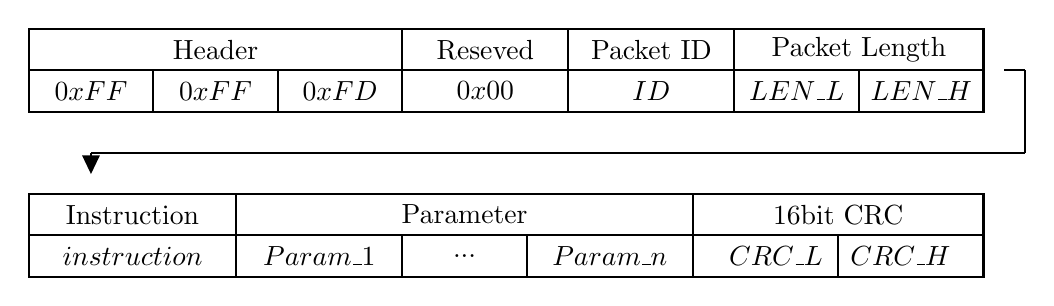
\begin{tikzpicture}[x=0.75pt,y=0.75pt,yscale=-1,xscale=1]
%uncomment if require: \path (0,158.99999237060547); %set diagram left start at 0, and has height of 158.99999237060547

%Shape: Rectangle [id:dp6250925726121845] 
\draw   (10,30) -- (70,30) -- (70,50) -- (10,50) -- cycle ;
%Shape: Rectangle [id:dp7150581119099197] 
\draw   (70,30) -- (130,30) -- (130,50) -- (70,50) -- cycle ;
%Shape: Rectangle [id:dp4157977425803503] 
\draw   (130,30) -- (190,30) -- (190,50) -- (130,50) -- cycle ;
%Shape: Rectangle [id:dp8588453097331337] 
\draw   (190,30) -- (270,30) -- (270,50) -- (190,50) -- cycle ;
%Shape: Rectangle [id:dp3240542971310183] 
\draw   (350,30) -- (410,30) -- (410,50) -- (350,50) -- cycle ;
%Shape: Rectangle [id:dp8255905540167148] 
\draw   (410,30) -- (470,30) -- (470,50) -- (410,50) -- cycle ;
%Shape: Rectangle [id:dp3504189874809429] 
\draw   (270,30) -- (350,30) -- (350,50) -- (270,50) -- cycle ;
%Shape: Rectangle [id:dp14784139403972163] 
\draw   (10,109.5) -- (110,109.5) -- (110,129.5) -- (10,129.5) -- cycle ;
%Shape: Rectangle [id:dp6901276280736819] 
\draw   (110,109.5) -- (190,109.5) -- (190,129.5) -- (110,129.5) -- cycle ;
%Shape: Rectangle [id:dp7962109651151303] 
\draw   (330,89.5) -- (470,89.5) -- (470,109.5) -- (330,109.5) -- cycle ;
%Shape: Rectangle [id:dp22518828865075857] 
\draw   (190,109.5) -- (250,109.5) -- (250,129.5) -- (190,129.5) -- cycle ;
%Shape: Rectangle [id:dp8071011784893514] 
\draw   (330,109.5) -- (400,109.5) -- (400,129.5) -- (330,129.5) -- cycle ;
%Shape: Rectangle [id:dp6565443085961074] 
\draw   (10,10) -- (190,10) -- (190,30) -- (10,30) -- cycle ;
%Shape: Rectangle [id:dp7685957084117421] 
\draw   (190,10) -- (270,10) -- (270,30) -- (190,30) -- cycle ;
%Shape: Rectangle [id:dp4215711805925242] 
\draw   (350,10) -- (470,10) -- (470,30) -- (350,30) -- cycle ;
%Shape: Rectangle [id:dp36748275994822155] 
\draw   (270,10) -- (350,10) -- (350,30) -- (270,30) -- cycle ;
%Shape: Rectangle [id:dp5326572155761315] 
\draw   (10,89.5) -- (110,89.5) -- (110,109.5) -- (10,109.5) -- cycle ;
%Shape: Rectangle [id:dp7964285396518918] 
\draw   (250,109.5) -- (330,109.5) -- (330,129.5) -- (250,129.5) -- cycle ;
%Shape: Rectangle [id:dp6204398584543338] 
\draw   (110,89.5) -- (330,89.5) -- (330,109.5) -- (110,109.5) -- cycle ;
%Shape: Rectangle [id:dp8858871341925003] 
\draw   (400,109.5) -- (470,109.5) -- (470,129.5) -- (400,129.5) -- cycle ;
%Straight Lines [id:da1982468191176332] 
\draw    (490,70) -- (40,70) ;


%Straight Lines [id:da9492408394597669] 
\draw    (40,70) -- (40,78) ;
\draw [shift={(40,80)}, rotate = 270] [fill={rgb, 255:red, 0; green, 0; blue, 0 }  ][line width=0.75]  [draw opacity=0] (8.93,-4.29) -- (0,0) -- (8.93,4.29) -- cycle    ;

%Straight Lines [id:da8759495506427029] 
\draw    (480,30) -- (490,30) ;


%Straight Lines [id:da5653929071720423] 
\draw    (490,30) -- (490,70) ;



% Text Node
\draw (40,40) node   {$0xFF$};
% Text Node
\draw (100,40) node   {$0xFF$};
% Text Node
\draw (160,40) node   {$0xFD$};
% Text Node
\draw (100,20) node  [align=left] {Header};
% Text Node
\draw (230,20) node  [align=left] {Reseved};
% Text Node
\draw (230,40) node   {$0x00$};
% Text Node
\draw (310,40) node   {$ID$};
% Text Node
\draw (310,20) node  [align=left] {Packet ID};
% Text Node
\draw (380,40) node   {$LEN\_L$};
% Text Node
\draw (440,40) node   {$LEN\_H$};
% Text Node
\draw (410,20) node  [align=left] {Packet Length};
% Text Node
\draw (60,119.5) node   {$instruction$};
% Text Node
\draw (60,100) node  [align=left] {Instruction};
% Text Node
\draw (150,119.5) node   {$Param\_1$};
% Text Node
\draw (220,119.5) node   {$...$};
% Text Node
\draw (290,119.5) node   {$Param\_n$};
% Text Node
\draw (220,99.5) node  [align=left] {Parameter};
% Text Node
\draw (370,119.5) node   {$CRC\_L$};
% Text Node
\draw (430,119.5) node   {$CRC\_H$};
% Text Node
\draw (400,99.5) node  [align=left] {16bit CRC};


\end{tikzpicture}

    \caption{Structure of the instruction packet}
    \label{fig:Instructsctruct}
\end{figure}
First, the instructional packet has a header field, which indicates the start of the packet. Then there is a reserved slot with the value $0x00$, note that $0xFD$ cannot be used.  The Packet ID, refers to the ID of the device that receives and process the sent data. In the next field information on the packet length is provided and after this is the instruction field. In this field, the purpose of the packet is defined.Hereafter the parameter fields is introduced, which contains help-data and are dependant on what instructions is in use. The last field contains the cycle redundancy check, which checks for errors in the data sent.  A list of further input can be seen in table \ref{tab:Instruct}.

\begin{table}[H]
\begin{tabular}{ | P{1.5cm} || P{2cm}|| P{9cm} |  }
 \hline
 \textbf{Value} & \textbf{Instruction} & \textbf{Description} \\
 \hline
 $0x01$ & Ping & Instruction that checks whether the Packet has arrived to a device with the same ID as Packet ID\\\hline
 $0x02$ & Read & Instruction to read data from the Device\\\hline
 $0x03$ & Write & Instruction to write data on the Device\\\hline
 $0x04$ & Reg Write & Instruction that registers the Instruction Packet to a standby status; Packet is later executed through the Action command\\\hline
  $0x05$ & Action & Instruction that executes the Packet that was registered beforehand using Reg Write\\\hline
  $0x06$ & Factory Reset & 	
Instruction that resets the Control Table to its initial factory default settings\\\hline
$0x08$ & Reboot & Instruction to reboot the Device\\\hline
$0x55$ & Status (Return) & Return Instruction for the Instruction Packet\\\hline
$0x82$ & Sync read & For multiple devices, Instruction to read data from the same Address with the same length at once\\\hline
$0x83$ & Sync Write & For multiple devices, Instruction to write data on the same Address with the same length at once\\\hline
 $0x92$ & Bulk Read & For multiple devices, Instruction to read data from different Addresses with different lengths at once\\\hline
  $0x93$ & Bulk Write & For multiple devices, Instruction to write data on different Addresses with different lengths at once\\\hline
\end{tabular}
\caption{Table of instructions Protocol 2.0\cite{PIDmxx}}
    \label{tab:Instruct}
\end{table}

\paragraph{The status packet} consists of the structure seen in the the figure below:
\begin{figure}[H]
    \centering
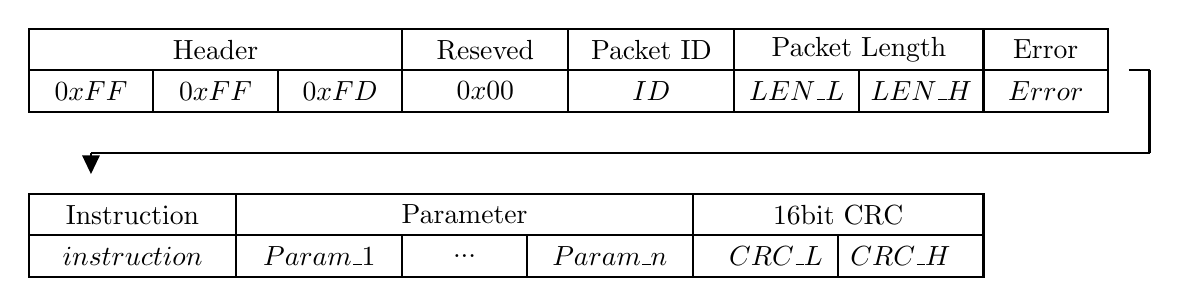
\begin{tikzpicture}[x=0.75pt,y=0.75pt,yscale=-1,xscale=1]
%uncomment if require: \path (0,158.99999237060547); %set diagram left start at 0, and has height of 158.99999237060547

%Shape: Rectangle [id:dp8698497909833363] 
\draw   (10,30) -- (70,30) -- (70,50) -- (10,50) -- cycle ;
%Shape: Rectangle [id:dp6485581117247297] 
\draw   (70,30) -- (130,30) -- (130,50) -- (70,50) -- cycle ;
%Shape: Rectangle [id:dp6658546174120246] 
\draw   (130,30) -- (190,30) -- (190,50) -- (130,50) -- cycle ;
%Shape: Rectangle [id:dp6752872057996913] 
\draw   (190,30) -- (270,30) -- (270,50) -- (190,50) -- cycle ;
%Shape: Rectangle [id:dp5014813538264575] 
\draw   (350,30) -- (410,30) -- (410,50) -- (350,50) -- cycle ;
%Shape: Rectangle [id:dp7457170593383808] 
\draw   (410,30) -- (470,30) -- (470,50) -- (410,50) -- cycle ;
%Shape: Rectangle [id:dp5054173748421811] 
\draw   (270,30) -- (350,30) -- (350,50) -- (270,50) -- cycle ;
%Shape: Rectangle [id:dp1263298518018401] 
\draw   (10,109.5) -- (110,109.5) -- (110,129.5) -- (10,129.5) -- cycle ;
%Shape: Rectangle [id:dp6896214683381987] 
\draw   (110,109.5) -- (190,109.5) -- (190,129.5) -- (110,129.5) -- cycle ;
%Shape: Rectangle [id:dp8350012688131694] 
\draw   (330,89.5) -- (470,89.5) -- (470,109.5) -- (330,109.5) -- cycle ;
%Shape: Rectangle [id:dp8375426281198146] 
\draw   (190,109.5) -- (250,109.5) -- (250,129.5) -- (190,129.5) -- cycle ;
%Shape: Rectangle [id:dp6586789788358929] 
\draw   (330,109.5) -- (400,109.5) -- (400,129.5) -- (330,129.5) -- cycle ;
%Shape: Rectangle [id:dp14973963332658702] 
\draw   (10,10) -- (190,10) -- (190,30) -- (10,30) -- cycle ;
%Shape: Rectangle [id:dp30939097077443956] 
\draw   (190,10) -- (270,10) -- (270,30) -- (190,30) -- cycle ;
%Shape: Rectangle [id:dp20452238276938295] 
\draw   (350,10) -- (470,10) -- (470,30) -- (350,30) -- cycle ;
%Shape: Rectangle [id:dp08631851455147288] 
\draw   (270,10) -- (350,10) -- (350,30) -- (270,30) -- cycle ;
%Shape: Rectangle [id:dp351731230245929] 
\draw   (10,89.5) -- (110,89.5) -- (110,109.5) -- (10,109.5) -- cycle ;
%Shape: Rectangle [id:dp46139057893485447] 
\draw   (250,109.5) -- (330,109.5) -- (330,129.5) -- (250,129.5) -- cycle ;
%Shape: Rectangle [id:dp42456037527605517] 
\draw   (110,89.5) -- (330,89.5) -- (330,109.5) -- (110,109.5) -- cycle ;
%Shape: Rectangle [id:dp5173327089860826] 
\draw   (400,109.5) -- (470,109.5) -- (470,129.5) -- (400,129.5) -- cycle ;
%Straight Lines [id:da19477344689590792] 
\draw    (550,70) -- (40,70) ;


%Straight Lines [id:da31415506805713345] 
\draw    (40,70) -- (40,78) ;
\draw [shift={(40,80)}, rotate = 270] [fill={rgb, 255:red, 0; green, 0; blue, 0 }  ][line width=0.75]  [draw opacity=0] (8.93,-4.29) -- (0,0) -- (8.93,4.29) -- cycle    ;

%Shape: Rectangle [id:dp13994941859002452] 
\draw   (470,10) -- (530,10) -- (530,30) -- (470,30) -- cycle ;
%Shape: Rectangle [id:dp04644653628071138] 
\draw   (470,30) -- (530,30) -- (530,50) -- (470,50) -- cycle ;
%Straight Lines [id:da3764266198993005] 
\draw    (550,70) -- (550,30) ;


%Straight Lines [id:da06827427289797416] 
\draw    (540,30) -- (550,30) ;



% Text Node
\draw (40,40) node   {$0xFF$};
% Text Node
\draw (100,40) node   {$0xFF$};
% Text Node
\draw (160,40) node   {$0xFD$};
% Text Node
\draw (100,20) node  [align=left] {Header};
% Text Node
\draw (230,20) node  [align=left] {Reseved};
% Text Node
\draw (230,40) node   {$0x00$};
% Text Node
\draw (310,40) node   {$ID$};
% Text Node
\draw (310,20) node  [align=left] {Packet ID};
% Text Node
\draw (380,40) node   {$LEN\_L$};
% Text Node
\draw (440,40) node   {$LEN\_H$};
% Text Node
\draw (410,20) node  [align=left] {Packet Length};
% Text Node
\draw (60,119.5) node   {$instruction$};
% Text Node
\draw (60,100) node  [align=left] {Instruction};
% Text Node
\draw (150,119.5) node   {$Param\_1$};
% Text Node
\draw (220,119.5) node   {$...$};
% Text Node
\draw (290,119.5) node   {$Param\_n$};
% Text Node
\draw (220,99.5) node  [align=left] {Parameter};
% Text Node
\draw (370,119.5) node   {$CRC\_L$};
% Text Node
\draw (430,119.5) node   {$CRC\_H$};
% Text Node
\draw (400,99.5) node  [align=left] {16bit CRC};
% Text Node
\draw (500,20) node  [align=left] {Error};
% Text Node
\draw (500,40) node   {$Error$};


\end{tikzpicture}

    \caption{Structure of the status packet}
    \label{fig:StatusStruct}
\end{figure}
\noindent
As seen, the only difference of the status packet, compared with the instructional packet, is the error field.
The error field indicates the result of the instruction packet. The error field can be seen in the figure below.\\ 
\begin{figure}[H]
    \centering
    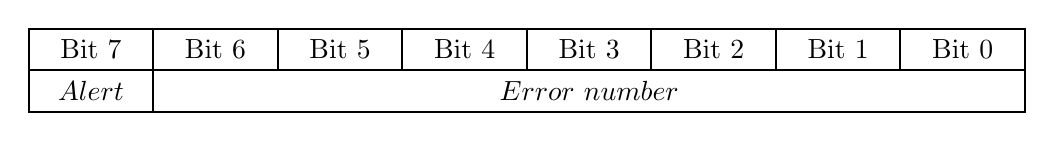
\begin{tikzpicture}[x=0.75pt,y=0.75pt,yscale=-1,xscale=1]
%uncomment if require: \path (0,158.99999237060547); %set diagram left start at 0, and has height of 158.99999237060547

%Shape: Rectangle [id:dp09142087079107619] 
\draw   (10,10) -- (70,10) -- (70,30) -- (10,30) -- cycle ;
%Shape: Rectangle [id:dp4629750443029259] 
\draw   (70,10) -- (130,10) -- (130,30) -- (70,30) -- cycle ;
%Shape: Rectangle [id:dp16194932941841267] 
\draw   (130,10) -- (190,10) -- (190,30) -- (130,30) -- cycle ;
%Shape: Rectangle [id:dp25658747620974176] 
\draw   (190,10) -- (250,10) -- (250,30) -- (190,30) -- cycle ;
%Shape: Rectangle [id:dp4454573381940983] 
\draw   (250,10) -- (310,10) -- (310,30) -- (250,30) -- cycle ;
%Shape: Rectangle [id:dp2107426327299584] 
\draw   (310,10) -- (370,10) -- (370,30) -- (310,30) -- cycle ;
%Shape: Rectangle [id:dp742699471984243] 
\draw   (370,10) -- (430,10) -- (430,30) -- (370,30) -- cycle ;
%Shape: Rectangle [id:dp768648200139064] 
\draw   (430,10) -- (490,10) -- (490,30) -- (430,30) -- cycle ;
%Shape: Rectangle [id:dp3416120520607919] 
\draw   (10,30) -- (70,30) -- (70,50) -- (10,50) -- cycle ;
%Shape: Rectangle [id:dp9451706315688295] 
\draw   (70,30) -- (490,30) -- (490,50) -- (70,50) -- cycle ;

% Text Node
\draw (40,20) node  [align=left] {Bit 7};
% Text Node
\draw (100,20) node  [align=left] {Bit 6};
% Text Node
\draw (160,20) node  [align=left] {Bit 5};
% Text Node
\draw (220,20) node  [align=left] {Bit 4};
% Text Node
\draw (280,20) node  [align=left] {Bit 3};
% Text Node
\draw (340,20) node  [align=left] {Bit 2};
% Text Node
\draw (400,20) node  [align=left] {Bit 1};
% Text Node
\draw (460,20) node  [align=left] {Bit 0};
% Text Node
\draw (40,40) node   {$Alert$};
% Text Node
\draw (280,40) node   {$Error\ number$};


\end{tikzpicture}

    \caption{Error structure\cite{PIDmxx}}
    \label{fig:Errorstruct}
\end{figure}
\noindent
In bit number 7, the alert changes the value from 0 to 1 if there is a failure on the device.\\
In table \ref{tab:StatusErrors}, different status errors can be seen.
\begin{table}[H]
    \centering
    \begin{tabular}{|P{1.5cm}||P{2cm}||P{9cm}|}\hline
       \textbf{Value}  & \textbf{Error} & \textbf{Description} \\ \hline
        $0x01$ & Result fail &  failed to process the sent Instruction Packet\\ \hline
        $0x02$ & Instruction Error &  undefined Instruction has been used OR Action has been used without Reg Write\\ \hline
        $0x03$ & CRC Error &  CRC of the sent Packet does not match\\ \hline
        $0x04$ & Data range Error &  Data to be written in the corresponding Address is outside the range of the minimum/maximum value\\ \hline
        $0x05$ & Data Length Error &  Attempt to write Data that is shorter than the data length of the corresponding Address\\ \hline
        $0x06$ & Data Limit Error &  Data to be written in the corresponding Address is outside of the Limit value\\ \hline
        
        $0x07$ & 
        Access Error&  Attempt to write a value in an Address that is Read Only or has not been defined OR  attempt to read a value in an Address that is Write Only or has not been defined OR attempt to write a value in the ROM domain while in a state of Torque Enable(ROM Lock)\\ \hline
    \end{tabular}
    \caption{Table of errors on the status packet}
    \label{tab:StatusErrors}
\end{table}




